% !TeX spellcheck = en_GB
\documentclass[11pt]{article}
\usepackage{amssymb}
\usepackage{latexsym}
\usepackage{amsmath}
\usepackage{amsthm}
\usepackage{stmaryrd}
\usepackage{fancyhdr}
\pagestyle{headings}
\usepackage{dsfont}
\usepackage{pifont}
\usepackage{mathtools}
\usepackage{natbib}
\usepackage{tikz-cd}
\usepackage{pgfplots}
\usepackage{enumitem} 
\usepackage{hyperref}
\usepackage{geometry}
\geometry{left=4cm,right=4cm}
\pgfplotsset{every axis/.append style={
		axis x line=middle,    % put the x axis in the middle
		axis y line=middle,    % put the y axis in the middle
		axis line style={<->}, % arrows on the axis
		xlabel={$x$},          % default put x on x-axis
		ylabel={$y$},          % default put y on y-axis
		ticks=none,
}}
%\usepackage[urw-garamond]{mathdesign}
%\usepackage{cmbright}
%\usepackage{concmath}
%\usepackage{sansmathfonts}
%\renewcommand*\familydefault{\sfdefault} %% Only if the base font of the document is to be sans serif

%\usepackage{pdfrender,xcolor,scrpage2}
%\pdfrender{StrokeColor=black,TextRenderingMode=2,LineWidth=1pt}
\tikzset{
	subseteq/.style={
		draw=none,
		edge node={node [sloped, allow upside down, auto=false]{$\subseteq$}}},
	Subseteq/.style={
		draw=none,
		every to/.append style={
			edge node={node [sloped, allow upside down, auto=false]{$\subseteq$}}}
	},
	Subsetneq/.style={
		draw=none,
		every to/.append style={
			edge node={node [sloped, allow upside down, auto=false]{$\subsetneq$}}}
	},
	Supseteq/.style={
		draw=none,
		every to/.append style={
			edge node={node [sloped, allow upside down, auto=false]{$\supseteq$}}}
	}
}

\hypersetup{
	colorlinks,
	citecolor=blue,
	filecolor=blue,
	linkcolor=blue,
	urlcolor=blue
}
\newtheorem{thm}{Theorem}[section]
\newtheorem{prop}[thm]{Proposition}
\newtheorem{lemma}[thm]{Lemma}
\newtheorem{cor}[thm]{Corollary}
\newtheorem{dfn}[thm]{Definition}
\newtheorem{axiom}[thm]{Axiom}
\newtheorem{rmk}[thm]{Remark}
\newtheorem{rmkt}[thm]{Remark by TeXer}
\newtheorem{ex}[thm]{Example}
\newtheorem{nex}[thm]{Non-example}
\newtheorem{exercise}[thm]{Exercise}
\newtheorem{question}[thm]{Question}
\newtheorem{problem}[thm]{Problem}
\newtheorem{dfn/thm}[thm]{Definition/Theorem}
\renewcommand{\baselinestretch}{1.1}
\renewcommand{\hom}{\text{ Hom}}
\newcommand{\spec}{\text{ Spec}\,}
\newcommand{\res}{\text{ res}}
\newcommand{\affn}{\mathbb A}
\newcommand{\proj}{\mathbb P}
\newcommand{\reals}{\mathbb R}
\newcommand{\cplx}{\mathbb C}
\newcommand{\intg}{\mathbb Z}
\newcommand{\bbf}{\mathbb F}
\newcommand{\ratl}{\mathbb Q}
\newcommand{\torus}{\mathbb T}
\newcommand{\sca}{{\mathfrak a}}
\newcommand{\scb}{{\mathfrak b}}
\newcommand{\scc}{{\mathfrak c}}
\newcommand{\scm}{{\mathfrak m}}
\newcommand{\scn}{{\mathfrak n}}
\newcommand{\scp}{{\mathfrak p}}
\newcommand{\scq}{\mathfrak q}
\newcommand{\frakg}{{\mathfrak g}}
\newcommand{\frakd}{{\mathfrak d}}
\newcommand{\calf}{{\cal F}}
\newcommand{\calg}{{\cal G}}
\newcommand{\cala}{{\cal A}}
\newcommand{\calb}{{\cal B}}
\newcommand{\calc}{{\cal C}}
\newcommand{\cale}{{\cal E}}
\newcommand{\cali}{{\cal I}}
\newcommand{\call}{{\cal L}}
\newcommand{\caln}{{\cal N}}
\newcommand{\calo}{{\cal O}}
\newcommand{\calr}{{\cal R}}
\newcommand{\mathbold}{\bf}
\newcommand{\cinf}{C^{\infty}}
\newcommand{\row}[2]{#1_1,\dots ,#1_{#2}}
\newcommand{\dbyd}[2]{{\partial #1\over\partial #2}}
\newcommand{\Space}{{\bf Space}}
\newcommand{\alg}{{\mathbold Alg}}
\newcommand{\notsubset}{\not \subset}
\newcommand{\notsupset}{\not \supset}
\newcommand{\pois}{{\mathbold Pois}}
\newcommand{\pd}{\partial}
\newcommand{\pitilde}{\tilde{\pi}}
\newcommand{\drta}{\dashrightarrow}
\newcommand{\rta}{\rightarrow}
\newcommand{\Lrta}{\Longrightarrow}
\newcommand{\lrta}{\longrightarrow}
\newcommand{\llrta}{\longleftrightarrow}
\newcommand{\Llta}{\Longleftarrow}
\newcommand{\Llrta}{\Longleftrightarrow}
\newcommand{\lgl}{\langle}
\newcommand{\rgl}{\rangle}
\newcommand{\inj}{\hookrightarrow}
\newcommand{\surj}{\twoheadrightarrow}
\newcommand{\cmark}{\ding{51}}%
\newcommand{\xmark}{\ding{55}}%
\newcommand{\downmapsto}{\rotatebox[origin=c]{-90}{$\scriptstyle\mapsto$}\mkern2mu}
\renewcommand{\qedsymbol}{$\square$}
\bibliographystyle{plain}
\title{\bf Lecture Notes for Algebraic Geometry I}
\author{Lecture delivered by Emmanuel Kowalski\\
Notes by Lin-Da Xiao and David Burgschweiger}
\date{2018 ETH} 
%\thanks{Research partially supported by NSF Grant DMS-96-25122 and the Miller Institute for Basic Research in Science.}
\begin{document}
\maketitle
\tableofcontents
\section*{About the notes}
In this notes we mainly focus on the algebraically closed fields.
\newpage
\section{Classical varieties}
\subsection{Feb 27th: Algebraic sets and morphisms}
\href{https://imaginary.org/programs}{https://imaginary.org/programs}

Recall: $V(I)\subset \affn^n =\{x|\forall f\in I, f(x)=0\}$.
\begin{dfn}
Closed subspaces of $\affn^n$ are called \textbf{affine algebraic sets} and irreducible algebraic sets are called \textbf{affine algebraic varieties}
\end{dfn}
\begin{dfn}
Given $Y$ an affine algebraic set in $\affn^n$, we define the \textbf{coordinate ring} $\calo(Y)$ as $K[X_1,...,X_n]/I(Y)$
\end{dfn}
\begin{dfn}
Let $X\subset \affn^m$ and $Y \subset \affn^n$ be affine algebraic sets. A \textbf{morphism} $X \lrta Y$ of affine algebraic sets is a map $f : X \lrta Y$ of the underlying sets such that there exist polynomials $f_1,...,f_n \in k[T_1,...,T_m]$ with $f(x) = (f_1(x),...,f_n(x))$ for all $x\in X$. 
\end{dfn}
We denote the category of affine algebraic sets over $K$ as $Alg_K$
\begin{thm}\label{thm:equivalence_of_categories_algebraic_sets_K_algebras}
Let $Y_1\subset \affn^n, X_1,...,X_n$, $Y_2\subset \affn^m, T_1,,..., T_m$ affine algebraic sets. There are bijections 
$$
\begin{aligned}
&\hom_{K\text{-alg}}(\calo(Y_2),\calo(Y_1))
\\
&\overset{(*)}{\llrta}\{(f_1,...,f_m)\in K[X]^m|\forall x\in Y_1,(f_1(x),...,f_m(x))\in Y_2) \}\\
&\overset{(**)}{\llrta} \{f:Y_1\lrta Y_2|\forall \varphi\in \calo(Y_2),\varphi\circ f\text{ is  in }  \calo(Y_1)\}\\
&=\hom_{Alg_K}(Y_1,Y_2)
\end{aligned}
$$
\end{thm}
\begin{proof}
\underline{Key observation}

To give $(f_1,...,f_m)\in K[X]^m$ is ``the same '' as giving a ring morphism $g_0:K[T]\lrta K[X]: T_i\mapsto f_i$, which gives by composition $g_1=\pi_1\circ g_0$, where $\pi_1: K[X]\lrta \calo(Y_1)$ is the canonical projection.
$$
g_1: K[T]\lrta \calo(Y_1)
$$
which has a factorization
\[
\begin{tikzcd}
K[T] \arrow[r,"g_1"] \arrow[d,"\pi_2"]  & \calo(Y_1)  \\
   \calo(Y_2) \arrow[ur,"g"] & 
\end{tikzcd}
\]
iff $g_1(I(Y_2))=0$, which means iff 
$$
g_1(\varphi)=\text{ ``replace $T_i$ by $f_i$ in $\varphi$''}
$$
belongs to $I(Y_1)$ if $\varphi\in I(Y_2)$, which means if $x\in Y_1$, then $g_1(\varphi)(x)=0$. That means $\varphi(f_1(x),...,f_m(x))=0$ for $\varphi\in I(Y_2),$ i.e., $(f_1(x),...,f_m(x))\in Y_2$. If $x\in Y_1$. In the statement, this gives the $(*)$ bijection. Any $k$-algebra morphism $\calo(Y_1)\lrta\calo(Y_2)$  comes from $K[T]\lrta \calo(Y_1)$ s.t. it vanishes on $I(Y_2)$.


For the bijection $(**)$, suppose 
$$
g:Y_1\overset{g}{\lrta} Y_2\overset{\varphi}{\lrta} K
$$
sends $\varphi(Y_2)$ to $\varphi\circ g\in\calo(Y_1)$. Then we get 
$$
\begin{aligned}
& \calo(Y_2)\lrta \calo(Y_1)\\
&\varphi\longmapsto \varphi\circ g,
\end{aligned}
$$
which is a $K$-algebra morphism.

As for the reverse direction, given $g$. From $\calo(Y_2)\lrta \calo(Y_1)$ to get a $g:Y_1\lrta Y_2$. We get a $\tilde{g}:Y_1\lrta Y_2$ in the second set
$$
\tilde{g}(x)=(f_1(x),...,f_m(x))
$$
then we have $\varphi\circ g\in\calo(Y_1)$ for $\varphi\in \calo(Y_2)$. One checks that this shows that the first and third sets are the same.
\end{proof}

Define morphism $Y_1\lrta Y_2$ by the second(and third) set.  Composition in the obvious way and identity is a morphism.
$\Lrta$ get a category $(Alg_K)$ of affine algebraic sets over $K$.

\begin{cor}
$Y\mapsto \calo(Y)$, $g\mapsto [\varphi\mapsto \varphi\circ g]$ is a functor: $(Alg_K)\lrta (K\text{-Alg})^{opp}$.
\end{cor}

\underline{Facts}: The ``image'' of this functor is the category of finitely generated $K$-algebras which are reduced.
\begin{proof}
$A$ finitely generated reduced $K$-algebra. ($\exists n\geq 1$, so that $K[X_1,...,X_n]/I\cong A$). Then ``$A$ is reduced''$\Llrta$ $I$ is radical ideal.
$\Lrta A=\calo(V(I))$, where $V(I)\subset \affn^n$.
\end{proof}

\begin{cor}
There is a equivalence of categories between 
$$
(\text{Algebraic sets over $K$})\llrta (\text{finitely generated reduced } K\text{-Algebras}.)
$$
\end{cor}

\begin{ex}\ 
\begin{enumerate}[label=(\arabic*)]
\item $\affn^1\lrta V(Y^2-X^3-X^2)\subset \affn^2$, $t\mapsto (t^2-1,t(t^2-1))$
\item $\affn^1\lrta V(Y^2-X^3)\subset \affn^2$: $t\longmapsto (t^2,t^3)$ is a bijection but \underline{Not} an isomorphism.
\item Assume $K$ with characteristic $p>0$, $K\supset \mathbb{F}_p$. $Y=V(f_1,...,f_m)$ where $f_i\in \mathbb{F}_p[X]\subset K[X]$. Consider the morphism:
$$
\begin{aligned}
&Y\lrta Y\\
& (x_1,..,x_n)\longmapsto (x_1^p,...,x_n^p).
\end{aligned}
$$
It is bijective and homeomorphism but not an isomorphism if $dim(Y)\geq 1$.
\end{enumerate}
\end{ex}
\begin{prop}
$Y=V(I)\subset \affn^n$
\begin{enumerate}[label=(\arabic*)]
\item The points of $Y$ are in bijection with maximal ideals $I\subset \calo(Y)$ by 
$$
Y\ni x\longmapsto \{f\in \calo(Y)|f(x)=0\}
$$
\item We have a bijection 
$$
\calo(Y)\llrta \hom_{Alg_K}(Y,\affn^1)
$$
\end{enumerate}
\end{prop}
\begin{proof}
(1) $I_x:=Ker(\calo(Y)\lrta K)$, $f\mapsto f(x)$, since the evaluation map is surjective $[1\mapsto 1]$, we get an isomorphism 
$$
\calo(Y)/I_x\overset{\sim}{\lrta} K,
$$
so $I_x$ is maximal in $\calo(Y)$.

Conversely, if $I\subset \calo(Y)$ is maximal, we get $I=I'/I(Y)$ for $I'\subset K[X]$ maximal. 

Nullstellensatz says $\exists (x_1,...,x_n)\in\affn^n$ s.t., $I'=(X_1-x_1,...,X_n-x_n)$. 

Since $I'\supset I(Y)$, we get $(x_1,..,x_n)\in Y$. Then we check that $\calo(Y)\lrta\calo(Y)/I\cong K$ is just given by $f\mapsto f(x_1,...,x_n)$. That means $I=I_x$.

(2) We saw in~\ref{thm:equivalence_of_categories_algebraic_sets_K_algebras}, that there is a bijection between sets
$$
\hom_{Alg_k}(Y,\affn^1)\llrta \hom_{K-alg}(\calo(\affn^1),\calo(Y)).
$$
But $\hom_{K-alg}(\calo(\affn^1),\calo(Y))=\hom_{K-alg}(K[X],\calo(Y))\cong \calo(Y)$ (by $g:\calo(\affn^1)\lrta \calo(Y)$, $g\mapsto g(X)$)
\end{proof}
\section*{Projective Algebraic sets}

Projective sets can have a good notion of ``compactness''.

N.B. Any $Y\in (Alg_K)$ is \textbf{quasi-compact}( open cover have a finite subcover).

\begin{dfn}
$\proj^n_K=\proj^n$ can be either defined as 

``the set of  lines in $\affn^{n+1}$ that pass through the origin''

or

``the equivalence classes of points in $K^{n+1}\backslash \{0\}$ with the equivalence relation $x\sim y$ iff $x=\lambda y$ for some $\lambda \in K$'' and we use the notion $[x_0:...:x_n]$ for the equivalence class of $(x_0,..,x_n)$
\end{dfn}

These two definitions are equivalent: 

Given a line $l\in \affn^1\llrta $ hyperplane in $K^{n+1}$, corresponds to a equation
$$
a_0X_0+....+a_n X_n=0
$$
with at least one of $a_i$ non-zero.

Conversely, from $[x_0:..:x_n]$, we  we get the corresponding hyperplane/line trivially.


Notes the following fact:

$$
\proj^n=\cup_{0\leq i\leq n} H_i,
$$
where $H_i=\{[x_0,...,x_n]|x_i\neq 0\}$ and there is a bijection 
$$
\begin{aligned}
&H_i\lrta K^n\\
&[x_0:...:x_n]\longmapsto\left(\frac{x_0}{x_i},...,\widehat{\frac{x_i}{x_i}},..,\frac{x_n}{x_i}\right)\\
&
[y_1:...:y_{i-1}:1:y_{i}:...:y_n]\mapsfrom(y_1,...,y_n)
\end{aligned}
$$
We define from linear algebra some notions in $\proj^n$ a line in $\proj^n$ is the image by the projection $K^{n+1}\backslash \{0\}\lrta \proj^n$ of the two dimensional affine subspace.

\begin{ex}
$l_1,l_2\subset \proj^2$ lines $\l_1\cap l_2$ is a line if $l_1$ and $l_2$ are identical and would be a single point otherwise.
\end{ex}

Observation: If $f\in K[X_0,...,X_{n+1}]$ is homogeneous, then for $x\in \proj^n$, it makes no sense to speak of ``$f(x)\in K$'', but the zero-loci or the set where $f(x)\neq 0$ does make sense.

\begin{dfn}
 A  \textbf{projective algebraic set} $S\subset \proj^n$ is 
 $$
  S=\{ x\in \proj^n|f_1(x)=...=f_m(x)=0\},
 $$
 where $f_1,...,f_m$ are homogeneous of some degrees.

 An irreducible projective algebraic set is called a \textbf{projective variety}
\end{dfn}

\underline{Notation}: $V(f_1,..,f_n)$

\begin{ex}
$V(Y^2 Z-X^3-X Z^2)\subset \proj^2$. 
\end{ex}
Let $0\leq i\leq n$, then $S\cap H_i=\{[x_0:...:x_n]\in S| x_i\neq 0\}$ is , via the bijection  $H_i\lrta K^n$, in bijection with an affine algebraic set $S_1\subset \affn^n$ given by $\tilde{f_1}(y)=...=\tilde{f}_m(y)=0$, where $\tilde{f}_i(y_1,..,y_n)=f_i(y_1,...,y_{i-1},1, y_i,...,y_n)$


\subsection{Mar 2nd: Projective algebraic sets and regular functions}
Recall: $\proj^n_K=K^{n-1}-\{0\}/\sim$, and $H_i:=\{[x_0:...:x_n]|x_i\neq 0\}$ is in bijection with $\affn^n$. $V(f_1,...,f_m)=\{x\in \proj^n|\forall i,f_i(x)=0\}$, where $f_1,..f_m$ are homogeneous.

More generally, we can define 
$$
V(I)=V(\text{homogeneous element of $I$=})=V(\cup_{d\geq 0} I_d)
$$
where $I$ is an homogeneous ideal of $K[X_0,...,X_n]$ that is  $I=\oplus_{d\geq 0} I_d$, $I_d$ the the degree $d$ piece of $K[X_0,...,X_n]$.

Conversely, given $S\subset \proj^n$, we can define 
$$
I(S):=\text{ideal generated by homogeneous polynomials that vanishes on $S$}
$$
\begin{lemma}
This is a homogeneous ideal
\end{lemma}
\begin{proof}
$f\in I(s)\Lrta f=\sum_{i\in I}g_i f_i$, where $f_i$ is homogeneous and vanishes on $S$. We can expand each $g_i$ as $\sum_j g_{ij}$, where each $g_{ij}$ is homogeneous in $I(S)$. Then we know $f\in \otimes I(S)_d$ and the converse is clear.
\end{proof}
\begin{lemma}
The projective sets $V(I)$ where $I$ is homogeneous form the closed sets of a topology. It is called the Zariski topology (same name for the induced topology on projective sets).
\end{lemma}
\begin{ex}
$H_0\subset \proj^n$ and $\sigma: H_0\cong \affn^n$. Under this bijection, the Zariski topologies correspond $\sigma $ is a homeomorphism
$$
f\in K[X_0,...,X_n]\text{ homogeneous} \leadsto V(f)\subset \proj^n
$$
$$
\tilde{f}=f(1,X_1,...,X_n)\in K[X_1,..,X_n]\leadsto V(\tilde{f})\subset \affn^n
$$
and $\sigma(V(f))=V(\tilde{f})$.
\end{ex}
\begin{dfn}
$Y\subset \proj^n$ projective $S(Y)=K[X_0,...,X_n]/I(Y)$, \textbf{homogeneous coordinate ring}
\end{dfn}
\underline{Note} elements in $S(Y)$ are not functions on $Y$. The geometric meaning of $S(Y)$ will be explained latter with the language of schemes.

We now want to define morphisms of  projective algebraic sets. We have to look at it more carefully because we can not simply copy the affine definition.
\begin{dfn}
$Y\subset \proj^n$ projective, let $V\subset Y $ be an open subsets of $Y$.
\begin{enumerate}[label=(\arabic*)]
\item $f: V\lrta K$ continuous is called \textbf{regular} on $Y$ if $\forall x\in Y$, $\exists U$ open $x\in U$, $\exists f_1,f_2\in K[X_0,...,X_n]$ homogeneous of same degree such that $f_2(x)\neq 0$ for all $x\in U$ and $f(x)=\frac{f_1(x)}{f_2(x)}$ for $x\in U\cap Y$
\item $Y_1,Y_2$ are projective sets in $\proj^n,\proj^m$, $f: Y_1\lrta Y_2$ is a \textbf{morphism} if $f$ is continuous and for any $U\subset Y_1$ open and any $\varphi:U\lrta K$ regular, the composite $\varphi\circ f: f^{-1}(U)\lrta K$ is regular.
\end{enumerate}
\end{dfn}
\underline{Note}: IN $(2)$, one can not restrict to $\varphi$ regular on $Y_2$ because often the space of such function is reduced to $K$
\begin{prop}
For $\proj^n$, the space of functions regular on $\proj^n$ is $K$.
\end{prop}
\begin{proof}
The case $n=1$ implies the general case: if $f:\proj^n\lrta K$ regular, and $x\neq y$ in $\proj^n$, the line joining $x$ to $y$ in $\proj^n$ is ``isomorphic'' to $\proj^1$ and $f|_L$ is regular so constant, hence $f(x)=f(y)$.

For $n=1$, suppose $x$, $y$ are arbitrary points and let $U \ni x$, $V\ni y$ be open neighbourhoods such that $f|_U =f_1(x)/f_2(x)$ and $f|_V = g_1(x)/g_2(x)$ where $f_1$, $f_2$, $g_1$, $g_2$ are homogeneous polynomials and $f_1$, $f_2$ have the same degree as well as $g_1$, $g_2$. We may assume that $f_1$ and $f_2$ are coprime and also $g_1$, $g_2$ are coprime. Hence on $U \cap V$,
$$
f_1 g_2 = g_1 f_2.
$$
We know that $U \cap V$ is infinite so this implies $f_1 = g_1$ and $ f_2 = g_2$. Since $x$ and $y$ were arbitrary points we conclude that $f = f_1(x)/f_2(x)$ on all of $\proj^1$ hence $f$ is a constant.
\end{proof}
\underline{Concretely}: To say that $f: Y_1\subset \proj^n\lrta Y_2\subset \proj^m$  is a morphism of projective algebraic sets. It reduces to 
$\forall x\in Y_1,\exists U$ open containing $x$ s.t. there exists $f_0,...,f_m\in K[X_0,...,X_{n+1}]$
homogeneous of same degree, with no common zero in $U$, such that
$\forall y\in U\cap Y_1$, $f(y)=[f_0(y):...:f_m(y)]$. It is easy to see that if $f$ is of this form, then it is a morphism.

The converse is left as an exercise.

\begin{ex}
\begin{enumerate}[label=(\arabic*)]
\item Let $g\in Gl_n(K), n\geq 1$. Define 
$$
f_g:\proj^n\lrta \proj^n
$$
$$
[x_0:...:x_n]\longmapsto [g(x_0,...,x_n)]
$$
is a morphism. In fact, it is an isomorphism. $f^{-1}_g=f_{g^{-1}}$.
It also has some other properties: $f_{g}=f_{\lambda g},\lambda\neq 0$ and we get an induced group morphism
\[
\begin{tikzcd}
PGL_{n+1}(K) \arrow[d] \arrow[r, equal] & GL_{n+1}(K)/K^\times \\
Aut_{proj}(\proj^n) & 
\end{tikzcd}
\]
which is an isomorphism. A special case is $Aut_{hol}(\cplx \proj^1)=PGL_2(\cplx)$
$$
g\longmapsto \left[z\mapsto \frac{az+b}{cz+d}\right]
$$
\item  $K=\cplx$. One can do  holomorphic geometry (using holomorphic functions instead of polynomials). IN $\cplx^n$,we get a  much more complicated picture [e.g. $V(\sin z)$] is a an infinite sets in $\proj^n_\cplx$, however Chow proved that the holomorphic sets and the projective algebraic sets are the same (Serre ``GAGA'' principle compares many different invariant of both categories.)
\item Consider the map $S:=V(Y^2Z-X^3-XZ^2)\overset{f}{\lrta} \proj^1$, $[x:y:z]\mapsto [y:z]$. \\
\underline{Claim}, this is a morphism of projective sets.
\\
This means that there is no solution to $Y^2Z-X^3-XZ^2=0$ with $Y=Z=0$. (But $[x:y:z]\mapsto [x:z]$ is not a morphism because $[0:1:0]\in S$). $f$ is surjective but not injective $[x:y:z]$ and $[x:-y:z]$ have same image. This works in field $k$ with $\text{char} k\neq 2$.
\item $\proj^1\overset{v}{\lrta} \proj^2$, $[x:y]\mapsto [x^2:xy:y^2]$ (special case of Veronese embedding). This is a morphism. The image of $v$ is equal to $[y_0:y_1:y_2], \proj^2$. $S=V(Y_1^2-Y_0Y_2)$.  In fact, $\sigma$ gives an isomorphism
$\sigma: \proj^1\lrta S$ with inverse given by 
$$
\tau: S\lrta \proj^1
$$
$$
[y_0:y_1:y_2]\mapsto\left\{\begin{matrix*}
&[Y_1:Y_2] \text{ if } Y_2\neq 0\\
&[Y_0:Y_1]\text{ if } Y_0\neq 0
\end{matrix*}
\right.
$$
$\tau$ is a morphism defined on all of $S$, because if $[y_0:y_1:y_2]\in S$ satisfies $y_0=y_2=0$, it would implie $y^2_1=y_0y_2=0\Lrta y_1=0$ 
$$
\begin{aligned}
\tau\circ \sigma([x:y])&=\tau([x^2:xy:y^2])
&=\left\{\begin{matrix*}
&[xy:y^2]=[x:y], y\neq 0
\\
&[x^2:xy]=[x:y], x\neq 0
\end{matrix*}\right.
\end{aligned}
$$
therefore $\tau\circ \sigma= id_{\proj^1}$ and $\sigma\circ \tau=id_S$ can proved similarly

One can not find $f_0:f_1$ in $K[Y_0,Y_1,Y_2]$ s.t. $\tau([y_0:y_1:y_2]=[f_0(Y):f_1(Y)]$ for all $Y\in S$
\end{enumerate}
\end{ex}

\subsection{Mar 5th: Exercise class}
The content covered can be found in Hartshorne, p50ff Proposition 7.4 and Theorem 7.5.


\subsection{Mar 6th: Rational/birational maps}

$Y\subset \affn^n$ algebraic if $Y$ is irreducible, then $\calo(Y)$ is an integral domain. Let $K(Y)$ be its quotient field. What is the geometric meaning of $K(Y)$? It is called the \textbf{function field} of $Y$.

We will see
\begin{thm}
For $Y_1,Y_2$ affine varieties (irreducible) $K(Y_1)\cong K(Y_2)$ as fields

$\Llrta$ $\exists U_1\subset Y_1$ open dense subset and $\exists U_2\subset Y_2$ open dense subset such that $U_1$ and $U_2$ are isomorphic.
\end{thm}
\begin{dfn}
(Quasi-affine  and quasi-projective) varieties)
\begin{enumerate}%[label=(\arabic*)]
  \item \textbf{quasi-affine variety} $V$ is an open subset $V\subset Y$, where $Y\subset \affn^n$ is an affine variety. $[V\neq \emptyset\Lrta V\text{ dense in } Y\Lrta V\text{ irreducible }]$. It is given by the Zariski's topology from $Y$.\\
  (1') $V\subset Y\subset \proj^n$ where $V$ is an open subset of $Y$ is \textbf{quasi-projective}, where $Y$ is projective variety.
  \item A regular function $f:V\lrta K=\affn^1$, where $V$ is quasi-affine is an $f$ such that for all $x\in V$, $\exists U\subset V$ open containing $x$ s.t., $\forall x\in V$, $f(x)=\frac{f_1(x)}{f_2(x)}$ where $f_1,f_2\in\calo(\affn^n)$ and $f_2(x)\neq 0$ on $U$.\\
  (2') $V$ is quasi-projective variety a regular function $f$ is $\frac{f_1(x)}{f_2(x)}$ $f_i$ homogeneous of same degrees.
  \item If $V_1,V_2$ are \underline{Varieties} (of any of the four types), then $f:V_1\lrta V_2$ is a \textbf{morphism} if for al open $U\subset V_2$ all $\varphi:U\lrta K$ regular, the composition $\varphi\circ f: f^{-1}U\lrta K$ is also regular.
  \end{enumerate}
\end{dfn}

N.B. \begin{enumerate}
\item This makes sense because if $U\subset V_2$, where $V_2$ is quasi affine $U$ open, $\Lrta$ $U\subset V_2\subset Y$ so $U$ is also quasi-affine in $\affn^n$
\item \underline{Exercise} If $f$ is regular on $V$, then $f$ is continuous $V\lrta \affn^1$. (check that $f^{-1}(\{a\})$ is closed, use that closedness is a local condition.)
\item In the (quasi)-affine case, it is enough to check that $\varphi\circ f$ is regular on $V_1$ for $\varphi$ regular on $V_2$.
\item \underline{Notation}:
$$\calo(V)=\{f:V\lrta K|\text{ regular}\}$$
This is a ring of with unity, and because of the condition that for open $V\subset Y$ in a variety $Y$, either $\calo(V)=0,V\neq \emptyset$ or $V$ is dense in $Y$, $\Lrta \calo(V)$ integral domain. 
\end{enumerate}

\begin{ex}\ 
\begin{enumerate}
\item $GL_n(K)=\{x\in M_{n\times n}(K)|\det(x)\neq 0\}\subset \affn^{n^2}$ is quasi-affine since $\det:M_{n\times n}(K)\lrta K$ is continuous and not emptyset.

\item In fact, for any $0\neq f\in \calo(\affn^n)$
$$
U_f=\{x\in \affn^n|f(x)\neq 0\}
$$
is a quasi-affine variety.

\underline{Fact}: There is an isomorphism
$$
\sigma = 
\left\{\begin{aligned}
U_f&\lrta Y=\{(x,y)\in\affn^{n+1}|yf(x)=1\}\\
x&\longmapsto \left(x,\frac{1}{f(x)}\right)
\end{aligned}
\right.
$$
with inverse
$(x,y)\overset{\pi}{\longmapsto}x$.
(Indeed, $\pi\circ \sigma=Id_{U_f}$, $\sigma\circ \pi=Id_Y$) and $\pi$ is a morphism: Consider $\varphi\in\calo(U_f)$
$$
Y\overset{u}{\lrta}U_f\overset{\varphi}{\lrta}K
$$
then $\varphi\circ \pi(x,y)=\varphi(x)$.

Indeed, for any $x\in U_f$, $\exists f_1,f_2\in \calo(\affn^2)\varphi(x)=\frac{f_1(x)}{f_2(x)}, f_2(x)\neq 0$, one can show: assume $f_2(x)=f(x)^d$ then 
$$
\varphi(x)=\frac{f_1(x)}{f(x)^d}=f_1(x)y^d
$$
for $(x,y)\in Y$, so this is regular.

(2) $\sigma$ is a morphism
$$
U_f\overset{\sigma}{\lrta}Y\overset{\varphi}{\lrta}K
$$
$\varphi\in\calo(Y)=K[X_1,...,X_n,Y]/(Yf(x)=1)$
$$
\begin{aligned}
\varphi\circ \sigma(x)&=\varphi(x,1/f(x))=\left(\sum_j a_j Y^j\right)|_{Y=1/f(X)}\\
&=\sum_j a_j (x)/f(x)^j\in \calo(U_f)
\end{aligned}
$$
\item $\proj^n=\cup_{0\leq i\leq n}H_i$, with $H_i=\{[x_0:...:x_n]|x_{i}\neq 0\}$, $H_i\subset \proj^n\}$ open , so quasi-projective. The map
$$
\left\{\begin{aligned}
H_i&\overset{f_i}{\lrta} \affn^n\\
[x_0:...:x_n]&\longmapsto (\frac{x_0}{x_1},...,\frac{x_{i-1}}{x_i},\frac{x_{i+1}{x_i}},...,\frac{x_n}{x_i})
\end{aligned}
\right.
$$
is an isomorphism.
\end{enumerate}
\end{ex}

\begin{dfn}
$Y$ variety, $K(Y)=\{(U,f)|\emptyset\neq U\subset Y\text{ open },f\in \calo(U)\}/\sim$, where $(U_1,f_1)\sim (U_2,f_2)$ iff $f_1|_{U_1\cap U_2}=f_2|_{U_1\cap U_2}$
\end{dfn}

\underline{Fact}: $\sim$ is an equivalence relation. We define
$$
(U_1,f_1)+(U_2,f_2)=(U_1\cap U_2,f_1+f_2)
$$
$$
0:=(Y,0),\ \ 1:=(Y,1)
$$
\begin{prop}
$Y$ is quasi-affine, $U\subset Y$ open nonempty.
\begin{enumerate}
\item $\calo(Y)\inj\calo(U)\inj K(Y)$\\
$f\longmapsto f|_U\mapsto (U,f)$
\item $K(Y)$ is a field, and identifies with the fraction field of $\calo(Y)$ and of $\calo(U)$.
\item if $Y$ is an affine variety, then $\calo(Y)$ as defined above coincides with $\calo(Y)=K[X_1,...,X_n]/I(Y)$ as defined in previous sections.\\

(3') If $Y=U_f$ for $0\neq f$ in $\calo(\affn^n)$, then $\calo(Y)=\{f_1/f^d|f_1\in \calo(\affn^n, d\geq 0\}=\calo(\affn^n)_f$ the localization at $f$.
\end{enumerate}
\end{prop}
\begin{proof}
(1), The morphism $\calo(Y)\lrta \calo(U)\lrta K(Y)$ are injective because any $U\subset Y,\neq \emptyset$ is dense.

(2) Let $(U,f)\neq 0$ in $K(Y)$, then $\exists x_0\in U$, $f(x_0)\neq 0$ in a $V\subset U$, $x_0\in V$
$$
f(x)=\frac{f_1(x)}{f_2(x)}, f_1,f_2\in\calo(\affn^n), f_2\neq 0\text{ in }V
$$
in particular, $f_1(x_0)\neq 0$ and $( U\cap\{f_1(x)\neq 0\},\frac{f_2(x)}{f_1(x)})\in K(Y)$, where $U\cap\{f_1(x)\neq 0\}\neq \emptyset$ is the inverse of $(U,f)$ in $K(Y)$. 

By $(1)$, $K(Y)\supset \calo(Y)$.

Let $(U,f)\in K(Y)$, pick $x\in Y$ so that around $x$, $f(x)=\frac{f_1}{f_2}$, $f_i\in\calo(\affn^n)$, then $(U,f)=\frac{(Y,f_1)}{(Y,f_2)}$, so $K(Y)$ is the fraction field of $\calo(Y)$.

(3) Write $\calo'(Y)=K[X]/I(Y)$.  Note $K[X..,Y]/I(Y)$ identifies to a ring of functions on $Y$, the claim is that this ring is $\calo(Y)$.

Observation:
For $x\in Y$, to say that $f: Y\lrta K$ is ``regular at $x$'' means precisely that $f\in \calo'(Y)_{I_x}$, where $I_x=\{f\in\calo'(Y)|f(x)=0\}$. (Localization at  a maximal ideal)

So $$
\begin{aligned}
\calo(Y)&=\bigcap_{x\in Y}\calo'(Y)_{I_x}\\
&=\bigcap_{\scm\subset\calo'(Y)}\calo'(Y)_\scm\\
&=\calo'(Y)
\end{aligned}
$$
the second equality from Nullstellensatz and the third from commutative algebra.

(3') Similarly, using characterization of maximal ideals in $A_f, f\neq 0$
\end{proof}

\begin{dfn}
K(Y) is called the fraction or function field of $Y$
\end{dfn}

\begin{ex}
$K(\affn^n)=K(\proj^n)=K(X_1,..,X_n)$
\end{ex}

\begin{dfn}
(Rational maps) $Y_1,Y_2$ varieties. A \textbf{rational map} $f: Y_1\dashrightarrow Y_2$ is a pair $(U,\tilde{f})$ where $U\neq \emptyset$ in $Y_1$ and $\tilde{f}:U\lrta Y_2$ is a morphism with $(U,\tilde{f})=(U',\tilde{f}')$ iff 
$$
\tilde{f}|_{U\cap U'}=\tilde{f}'|_{U\cap U'}
$$
[Check: this is coherent, i.e., this is an equivalence relation]
\end{dfn}

\begin{dfn}
$f:Y_1\dashrightarrow Y_2$ is a \textbf{dominant} if its image $\tilde{f}(U)\subset Y_2$ is dense.
\end{dfn}

\begin{ex}\ 
(1) there is a bijection $\{Y\dashrightarrow \affn^1\}=K(Y)$
$$
\begin{matrix}
(U,\tilde{f}) & (U,f)\\
\tilde{f}:U\lrta \affn^1\text{ morphism } & f: U\lrta K\text{ regular}
\end{matrix}
$$
So it is enough to check 
$$
\hom_{Var}(U,\affn^1)=\calo(U)
$$
Left as exercise

(2) $Y,f_1,f_2,f_3\in\calo(Y)$
$$
\left\{\begin{aligned}
Y&\dashrightarrow \proj^2\\
x&\longmapsto [f_1(x):f_2(x):f_2(x)]
\end{aligned}\right.
$$
defined on $\{x|f_i (x) \text{ are not all zero}\}$, which is open if any of the $3$ sections is non-zero.
\end{ex}
\begin{thm}
$Y_1,Y_2$ varieties

$\exists \{Y_1\overset{f}{\dashrightarrow} Y_2|f \text{ dominant}\}$

$\overset{bij}{\llrta}$

$K(Y_2)\lrta K(Y_1)$
\end{thm}

\begin{cor}
$Y_1, Y_2$ varieties. $Y_1$ and $Y_2$ are birational 

iff $K(Y_1)$ is isomorphic to $K(Y_2)$

iff $\exists U\subset Y_1$ open $\neq \emptyset$
$\exists V\subset Y_2$, open $\neq \emptyset$ so that $U$ and $V$ are isomorphic as varieties.
\end{cor}

\begin{cor}
Any variety $Y$ of dimension $d\geq 0$ is birational to a hypersurface $V\subset \proj^{d+1}$
\end{cor}
\begin{proof}
(1) Given $Y_1\overset{f}{\dashrightarrow}Y_2$ dominant, we want a morphism
$K(Y_2)\lrta K(Y_1)$.

 Let $(U,\tilde{f})=f$, $(V,\varphi),\varphi:V\lrta K$ in $K(Y_2)$
$$
\varphi\circ f: \tilde{f}^{-1}(V)\lrta K
$$ 
 is in $K(Y_1)$, provided $\tilde{f}^{-1}(V)$ is dense, it is enough that $\tilde{f}^{-1}(V)\neq \emptyset$, $\tilde{f}(U)\cap V\neq \emptyset$, since $V$ is open and $\tilde{f}(U)$ is dense.

 (2) Given $i: K(Y_2)\lrta K(Y_1)$. Let $\tilde{Y_2}\subset Y_2\subset \affn^n$ open quasi-affine so that $K(Y_2)=K(\tilde{Y_2})=Frac(\calo(\tilde{Y}_2))$

 Let $X_1,..,X_n$ be the coordinates  in $\affn^n$ as elements of $\calo(\tilde{Y}_2)$, then let
 $$
f_j =i (X_j)\in K(Y_1)
 $$
 $f_j\llrta (U_j,\tilde{f}_j)$ with $U_j\subset Y_1$ dense and $\tilde{f}_j\in\calo(U_j)$. Then 
 $f_j\llrta (U,\tilde{f}_j)$, $U:=U_1\cap ...\cap U_n$ still dense.

 Define $U\lrta \tilde{Y}_2\inj Y_2$ by
 $$
x\longmapsto (\tilde{f}_1(x),...,\tilde{f}_n(x)).
 $$
This is a rational map $Y_1\dashrightarrow Y_2$

\end{proof}

\subsection{Mar 9th: Continue and Nonsingular varieties}

Recall
\begin{thm} $Y_1,Y_2$ varieties
$$\{ \text{dominant }Y_1\dashrightarrow Y_2\}\llrta\{K(Y_2\inj K(Y_1)\}$$
\end{thm}
\begin{cor}The followings are equivalent:
\begin{itemize}
	\item
$Y_1$  and $Y_2$ are birational \item the function field $K(Y_1)$ and $K(Y_2)$ are isomorphic
\item $\exists \emptyset \neq U\subset Y_1$, $\emptyset \neq V\subset Y_2$ and isomorphism between $U$ and $V$
\end{itemize}
\end{cor}
\begin{proof}
The last condition implies the second because $K(Y_1)=Frac(\calo(U))\cong Frac(\calo(V))=K(Y_2)$. Assume we have rational maps 
$$
Y_1\overset{f_2}{\drta}Y_2\overset{f_2}{\drta} Y_1
$$
with $f_2\circ f_1=id_{Y_1}, f_2\circ f_1= id_{Y_2}$. 

Let $f_1=(U',\tilde{f}_1), f_2=()V',\tilde{f}_2$
\[
\begin{tikzcd}
Y_1 \arrow[r, dashed,"f_1"] & Y_2 \arrow[r, dashed,"f_2"] & Y_1 \\
U' \arrow[ru, "\tilde{f}_1"'] \arrow[u,hook] & V' \arrow[ru, "\tilde{f}_2"'] \arrow[u, hook] & 
\end{tikzcd}
\]
$$
f_2\circ f_1=(Y_1,Id_{Y_1})
$$
so $\tilde{f}_2(\tilde{f}_1(x))=x$ if $\tilde{f}_1(x)\in V'$.
Similarly, $f_1\circ f_1=(\tilde{f}_2^{-1}(U'),\tilde{f}_1\circ \tilde{f}_2)$. Define $U=\tilde{f}^{-1}_{1}(\tilde{f}_{2}^{-1}(U'))\subset U'$, which is a dense open subset. Also we have $V=\tilde{f}^{-1}_{2}(\tilde{f}_{1}^{-1}(V'))$.

\underline{Claim}: $U\overset{\tilde{f}_1}{\lrta }V\overset{\tilde{f}_2}{\lrta} U$ and then $\tilde{f}_1|_U,\tilde{f}_2|_U$ are reciprocal isomorphism.

We check that if $x\in  U$, then $\tilde{f}_1(x)\in V$.
Let $y=\tilde{f}_1(x)\in V'$ so $\tilde{f}_2(y)=\tilde{f}_2(\tilde{f}_1(x))=x$ so $\tilde{f}_1(\tilde{f}_2(y))=\tilde{f}_1(x)\in V'$ $\Lrta y\in V$. Similarly for $f_2$.
\end{proof}

\begin{dfn}
A \textbf{rational variety} $Y$ is a variety $Y$ birational to $\proj^n$ for some $n$ (or to $\affn^n$). BY the theorem above we know $\exists n, K(Y)\cong K(X_1,...,X_n)$. 

A \textbf{unirational variety} $Y$ is a variety s.t. there is a dominant $\proj^n\drta Y$ for some $n$, by theorem above $\exists n, K(Y)\inj K(X_1,...,X_n)$
We obviously have
$$
\text{ Unirational } \Llta \text{rational}
$$
but 
$$
\text{ Unirational } \overset{?}{\Lrta} \text{rational}
$$
\end{dfn}
For $\text{char}= 0$: $\dim Y=1$ or $2$, Luroth and some italian showed that unirational curves or surfaces are rational.

First example in char $0$ of non-rational unirational varieties were provided by Clemens-Griffith: certain cubic hypersurfaces in $\dim 3$. 

Iskovskih-Manin ``general '' quantic hypersurfaces of $\dim 3$.

\begin{cor}
Any variety $Y$ is birational to a hypersurface in $\proj^{\dim(Y)+1}$ or $\affn^{\dim(Y)+1}$.
\end{cor}
\begin{proof}
Let $d=\dim(Y)=\dim(\calo(Y))$. Then a fact in commutative algebra says $K(Y)$ is a finite separable extension of $K(X_1,...,X_d)=:E$. By the primitive element theorem, there exists $\alpha:\in K(Y)$ such that  $K(Y)=E(\alpha)$. Let $f\in E[T]$ be the minimal polynomial of $\alpha$.

Write
$$
f=\sum_{i=0}^na_i T^i=\sum_{i=0}^n \frac{b_i}{c_i} T^i,
$$
where $a_i\in E$ and $a_i, b_i\in A=K[X_1,...X_d]$

$\Lrta$ $\tilde{f}(\alpha)=0$ where $\tilde{f}=\left(\prod c_i\right)f\in A[T]=K[X_1,...,X_d,T]$. Define $\tilde{Y}=V(\tilde{f})\subset \affn^{d+1}$. This is what we wanted.
\begin{enumerate}[label=(\arabic*)]
\item $\tilde{Y}$ is an irreducible hypersurface.
\item $\tilde{Y}$ is birational to $Y$ $\Llrta K(\tilde{Y})=K(Y)$
\end{enumerate}

\underline{Step 1}: Need $\tilde{f}_1\in K[X_1,...,X_d,T]$ irreducible. Suppose $\tilde{f}=\tilde{f}_1\tilde{f}_2, \tilde{f}_i\in A[T]\Lrta E\ni f=\frac{\tilde{f}_1}{\prod c_i}\tilde{f}_2 $ factors in $E[T]$, since $f$ is irreducible in  $E[T]$, one of $\deg(\tilde{f}_1)$ or $\deg(\tilde{f}_2)$ is zero

$\Lrta \tilde{f}$ is irreducible.

\underline{Step (2)}: $\calo(\tilde{Y})=K[X,T]/(\tilde{f})$. We have an injective morphism
$$
\left\{\begin{aligned}
 \calo(\tilde{Y})&\lrta K(Y)=E(\alpha)\\
 X_i&\longmapsto X_i\\
 T&\longmapsto \alpha
\end{aligned}
\right.
$$
so the fraction field $K(\tilde{Y})$ injects into $K(Y)$. The image of $K(\tilde{Y})$ contains $X_1,...,X_d$ and $\alpha$ hence it contains $E(\alpha)$, i.e., $K(\tilde{Y})=K(Y)$
\end{proof}

\section*{Nonsingular varieties}
Concrete geometric definition:
\begin{dfn}
$Y\subset \affn^n$ affine variety $\dim Y=d$, $x\in Y$. We say $Y$ is \textbf{nonsingular} at $x$ if for any generating set $\underline{f}:=(f_1,...,f_m)$ of $I(Y)$, the Jacobian matrix at $x$
$$
J_{\underline{f}}(x)=\left(\frac{\pd f_i(x)}{\pd x_j}\right)_{1\leq i\leq m, 1\leq j \leq n}\in M_{m\times n}(K)
$$
has rank $n-d$. If this holds for all $x$, then we say $Y$ is nonsingular.
\end{dfn}
\underline{Key fact}: It suffices to check the rank of $J_F(x)$ for some generating set. 

Indeed suppose $\underline{h}=(h_1,..,h_k)$ also generate $I(Y)$ so
$$
f_i = \sum^k_{\ell=1} g_{i\ell} h_\ell,
$$
where $g_{i\ell}\in \calo(\affn^n)$, $\frac{\pd f_i}{\pd x_j}=\sum^k_{\ell=1}\frac{\pd g_{i\ell}}{\pd x_j}h_\ell+\sum^k_{\ell=1}g_{i\ell}\frac{h_\ell}{x_j}$

At $x$ where $h_\ell(x)=0$, we get 
$$
\frac{\pd f_i}{x_j}(x)=\sum^k_{\ell=1}\frac{\pd g_{i\ell}}{\pd x_j}h_\ell
$$
$$
\Lrta J_{\underline{f}}(x)=M J_{\underline{h}}(x)
$$
so rank $J_{\underline{f}}(x)\leq \text{rank } J_{\underline{h}}(x)$. Exchanging $\underline{f},\underline{h}$, we get the equality.

\begin{ex}

\end{ex}\ 
\begin{enumerate}[label=(\arabic*)]
\item If $K=\cplx$, the implicit function theorem says that around a point where $J_{\underline{f}}(x)$ has rank $n-d$, then $V(f_1,...,f_m)$ is diffeomorphic to $\cplx^d$
\item Let $Y=V(f)$, $f$ irreducible in $\affn^n$. Then $x\in V(f)$ is nonsingular
$\Llrta(\pd f(x)/\pd x_1,...,\pd f(x)/\pd x_n)\neq 0$
\end{enumerate}


We have a singular point $\Llrta$ the system of $n+1$ equations 
$$
\left\{ \begin{aligned}
f(x)&=0\\
\frac{\pd f}{\pd x_1}(x)&=0\\
\vdots &\\
\frac{\pd f}{\pd x_n}(x)&=0
\end{aligned}\right.
$$
has a solution. 
For instance 
$$
Y^2=X^3
$$
\begin{center}
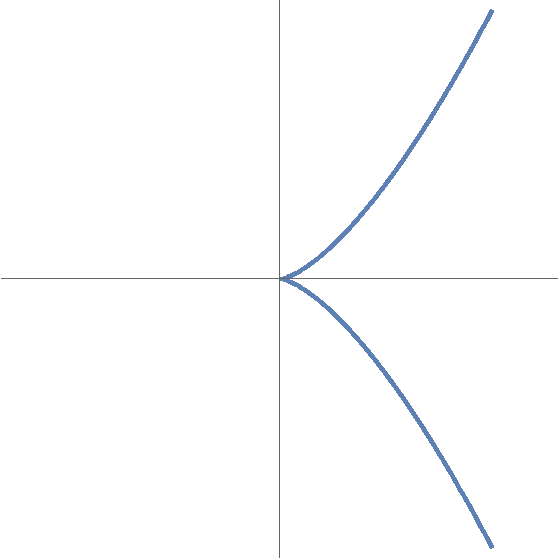
\includegraphics[scale=0.5]{Y^2-X^3}
\end{center}

$$
\left\{ \begin{aligned}
f&=Y^2-X^3\\
\frac{\pd f}{\pd X}&=-3X^2\\
\frac{\pd f}{\pd Y}&=2Y
\end{aligned}\right.
$$
so $X=Y=0$ is the only singular point.

$$Y^2=X^3-X$$
\begin{center}
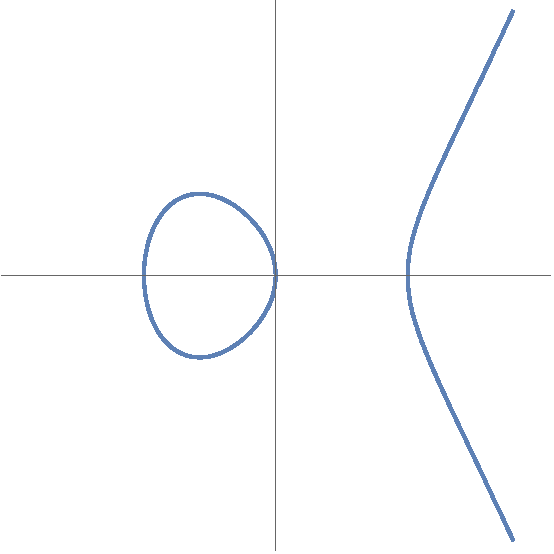
\includegraphics[scale=0.5]{Y^2=X^3-X}
\end{center}
$$
\left\{ \begin{aligned}
f&=Y^2-X^3+X\\
\frac{\pd f}{\pd X}&=-3X^2+1=0\\
\frac{\pd f}{\pd Y}&=2Y=0
\end{aligned}\right.
$$
If $\text{char }k\neq 2$, $\Lrta Y=0$, $X^3-X=0$ $X=0,-1,1$ do not satisfy the system of solutions. In the case $\text{char}=2$, $(1,0)\in Y$ is singular.


The intrinsic characterization was found by Zariski. 
\begin{dfn}
$x\in Y$ variety
\begin{enumerate}[label=(\arabic*)]
\item The \textbf{local ring} of $Y$ at $x$
$$
\begin{aligned}
\calo_{Y,x}&=\{f\in K(Y)|f\text{ defined  at } x\}\\
&=\{\text{ regular functions on some } U\ni x\}/(f_1\sim f_2\text{ if they coincide on } U_{f_1}\cap U_{f_2})
\end{aligned}
$$
if $Y$ is affine, then $\calo_{Y,x}=\{f_1/f_2\in K(Y) \mid f_i\in\calo(Y),f_2(x)\neq 0\}=\calo(Y)_{\scm_x}$, where $\scm_x=\{f\in\calo(Y)|f(x)=0\}$ is the maximal ideal corresponding to $x$.
$$
\calo(Y)\subset\calo_{Y,x}\subset K(Y)
$$
\end{enumerate}
\end{dfn}
\begin{dfn}
$Y\subset \affn^n$ affine $x\in Y$. The (Zariski) cotangent spaces of $Y$ at $x$ is the $K$-vector space
$$
\scm_{Y,x}/\scm_{Y,x}^2,
$$
where $\scm_{Y,x}\subset \calo_{Y,x}$ is the maximal ideal 
\end{dfn}
\begin{rmk}
$\calo_{Y,x}$ is a local ring, it has a unique maximal ideal $\scm$ which is $\calo_x\calo_{Y,x}$ in the affine case. Moreover $\calo_{Y,x}/\scm=K$ by $f\mapsto f(x)$.
\end{rmk}

N.B. Intuitively,  the Taylor expansion of $f\in \calo_{Y,x}$ about $x\in\scm_{Y,x}$ is
$$
f(X)=f(x)+\sum^n_{j=1}\frac{\pd f}{\pd x_j}(x)(X-x_j)+\dots
$$
if $f\in\scm_{Y,x}$ then $f(x)=0$ and terms of order $\geq 2$ belongs to $\scm_{Y,x}^2$, so $f$ has image
$$
\sum \frac{\pd f}{\pd x_j}dX_j\in \scm_{Y,x}/\scm_{Y,x}^2
$$
where $dX_j=X-x_j$.



\begin{dfn}
A local ring $\calo$ with maximal ideal $\scm$ is callled \textbf{regular} if 
$$
\dim \calo= \dim_k \scm/\scm^2
$$
where $k=\calo/\scm$ is the residue field.
\end{dfn}

\subsection{Mar 13th-A: Continue and proofs}
%Recall:
%$x\in Y\subset \affn^n$, $d=\dim(Y)$ affine variety,  and $Y$ is non-singular at $x$ iff 
%$$
%rank\ J_{\underline{f}}(x)=n-d.
%$$
\begin{thm}(Zariski)
	For $x\in Y\subset \affn^n$ the following are equivalent:
	\begin{enumerate}[label=(\arabic*)]
		\item
		$Y$ is non-singular at $x$
		\item $\dim(Y)=\dim_K(\scm_{Y,x}/\scm_{Y,x}^2)$, where $\scm_{Y,x}$ is the maximal ideal in the local ring $\calo_{Y,x}:=\calo(Y)_{\tilde{\scm}_{Y,x}}$ with $\tilde{\scm}_{Y,x}=\{f\in\calo(Y)\mid f(x)=0\}$.
	\end{enumerate}
\end{thm}


\begin{rmk}
	One can show $\dim_K\scm_{Y,x}/\scm_{Y,x}^2\geq \dim (Y)$ so the question is whether it is larger or not. 
\end{rmk}

\begin{proof}
	Denote $I:=I(Y)$, $d= \dim Y$ and  $x:=(x_1,...,x_n)\in\affn^n$.
	Let $I_x:=(X_1-x_1,...,X_n-x_n)\subset \calo(\affn^n)$ so that $\tilde{\scm}_{Y,x}=I_x/I$.
	There  is an isomorphism of $K$-vector spaces
	$$
	\theta:\left\{\begin{aligned}
	I_x/I_x^2&\lrta K^n\\
	f&\longmapsto \left(\frac{\pd f}{\pd X_j}(x)\right)_{1\leq j\leq n}
	\end{aligned}\right. .
	$$
	To see this, note that $f\in I^2_x$ iff $f=\sum_{i,j}h_{ij}(X_i-x_i)(X_j-x_j)$ and thus each $f \in I_x/I_x^2$ can be expressed as
	$$
	f=\sum_{i}^n(X_i-x_i)\frac{\pd f}{\pd X_i}(x)+I_x^2.
	$$
	That means each $f$ is uniquely defined by its derivatives and this preserves scalar multiplication.
	
	Let $(f_1,...,f_m)$ be a generating set of $I$. Then $(\theta(f_1),...,\theta(f_m))$ are the columns of $J_{\underline{f}}(x)$ and for any $f\in I$ we can write
	$$
	f=\sum_j g_j f_j
	$$
	for some $g_j \in K[X]$. Thus
	$$
	\frac{\pd f}{\pd X_i}(x)=\sum^n_{j=1} g_j(x)\frac{\pd f_j}{\pd X_i}(x).
	$$
	In vector notation this is
	$$
	\theta(f)_i=\sum^n_{j=1} g_j(x) \theta(f_j)_i .
	$$
	We conclude that the span of the $\theta(f_j)$ is $\theta((I+I_x^2)/I_x^2)$, so 
	$$
	rank\  J_{\underline{f}}(x)=\dim_K\theta((I+I_x^2)/I_x^2) = \dim_K (I+I_x^2)/I_x^2 .
	$$
	Consider the short exact sequence
	$$
	0 \lrta (I +I_x^2)/I_x^2  \lrta I_x/I_x^2 \lrta I_x/(I+I_x^2)  \lrta 0 .
	$$
	From this we see that 
	$$ rank \ J_{\underline{f}}(x) + \dim_K  I_x/(I+I_x^2) = \dim_K I_x/I_x^2 .$$  
	We already established that the RHS is $n$ hence $x$ is non-singular iff 
	$d=\dim_K I_x/(I+I_x^2)$. 
	
	Consider 
	$$
	\begin{tikzcd}
	I_x \arrow[r] \arrow[rr, "\varphi"', bend right] & \tilde{\scm}_{Y,x}\subset \scm_{Y,x} \arrow[r] & \scm_{Y,x}/\scm_{Y,x}^2
	\end{tikzcd}
	$$
	Note $\varphi(I+I_x^2)=0$ so we get a $K$-linear map 
	$$
	I_x/(I+I_x^2)\lrta \scm_{Y,x}/\scm_{Y,x}^2
	$$
	\underline{Claim}: This is an isomorphism $[\Lrta$ the theorem].  
	(a) $\varphi$ is surjective: 
	$h\in \scm_{Y,x}\subset \calo_{Y,x}\subset K(Y)$, $\Lrta h=\frac{h_1}{h_2}$, with $h_1, h_2\in\calo(Y)$ and $h_2(x)\neq 0, h_1(x)=0$. Then $$
	h-\frac{h_1}{h_2(x)}=h_1\left(\frac{h_2(x)-h_2}{h_2(x)h_2}\right)\in\scm_{Y,x}^2$$
	$$
	\Lrta [h]=\varphi\left(\frac{h_1}{h_2(x)}\right),
	$$
	where $\frac{h_1}{h_2(x)}\in I_x$, so $\varphi$ is surjective.
	
	(b) $\ker(\varphi)=I+I_x^2\subset I_x$ (Intuitively, the restriction of $f$ on $Y$ vanishes to order $2$ ar $x$). 
	
	\underline{Precisely}: 
	$$
	\calo_{Y,x}=(\calo(\affn^n)/I)_{I_x/I}=\calo(\affn^n)_{I_x}/I\calo(\affn^n)_{I_x}
	$$
	the last equality from commutative algebra. $\varphi(f)=0$ means that $f\mod I$ belongs to $(I_x^2)_{I_x}$ which is an ideal in $\calo(\affn^n)_{I_x}$ generated by $I_x^2$
	$$
	f\mod I=\sum_{i,j}(X_i-x_i)(X_j-x_j)h_{ij}
	$$
	$\theta(f\mod I)=0\Lrta f\in I+I_x^2$.
\end{proof}

\begin{thm}
Let $Y\subset \affn^n$ affine variety. Then $Y^\circ =\{x\in Y\mid Y\text{ non-singular at } x\}$  is dense open subset.
\end{thm}
\begin{cor}
Any variety $Y$ is birational to a non-singular variety.
\end{cor}
\begin{proof}
(of theorem)\\
Let $S=Y-Y^\circ=\{\text{ singular points }\}$. Then we know

$(1)$ $S$ is closed in $Y$, indeed fixing $(f_1,...,f_m)$ generating $I(Y)$
$$
S=\{x\mid rank\  J_{\underline{f}}(x)\neq n-d\} 
$$
One can show that $rank\ J_{\underline{f}}(x\leq n-d)$. So
$$
\begin{aligned}
S&=\{x\mid rank\  J_{\underline{f}}(x)< n-d\}\\
&=\{x\in Y\mid \text{ for all minors $M$ of $J_{\underline{f}}$ of size $n-d$ are degenerate $\det (M)=0$.}\}
\end{aligned}
$$
is a closed algebraic set in $\affn^n$.

$(b)$, $S\neq Y(\Lrta Y^\circ\neq \emptyset$ and open, so is dense). 

If $S=Y$, then by the theorem of Zariski, the set of non-singular points in an open set of a hypersurface birational to $Y$ would be empty. This means that we may assume $Y=V(f)\subset \affn^{d+1}$ with $f$ non-zero irreducible.
 Then 
 $$
V(f)\supset S=\left\{x\in \affn^{d+1}|0=f(x=\frac{\pd f}{x_1}(x)=...=\frac{\pd f}{x_d}(x)\right\}
 $$
 so if $S=V(f)$, $\frac{\pd f}{\pd x_1}\in I(V(f))=f\calo(\affn^{d+1})=f K[X_1,..,X_{d+1}]$
 $$
\Lrta \text{ in char }=0, \text{ comparing degrees, we have contradiction}
 $$
 $\Lrta$ in chat $p\neq 0$, we get $\frac{\pd f}{\pd x_i}=0$ for $1\leq i\leq d$,
 $\Lrta f\in K[x_1^p,..,X_d^{p}]\Lrta f=g^p$, contradicting the irreducibility.
\end{proof}
\section{Schemes}
In this chapter we will mainly follow chap 2 of Hartshorne and chap 1 of Eisenbud-Harris.
\subsection{Mar 13th-B: Affine schemes}
\subsubsection*{Motivations}
Serious problems with classical approach occur in late 1950's
\begin{enumerate}[label=(\arabic*)]
\item Intrinsic definitions (Without embeddings in $\affn^n$ or $\proj^n$)
\item Construction of various algebraic varieties especially Jacobian variety of a curve, especially w.r.t. base field (is the Jacobian of a curve given by equation with coefficients in the same field?)
\item Reduction modulo $p$ of a variety given by equation in $\intg[X_1,..,X_n]$
\end{enumerate}
To attack $(1)$, Serre started from
$$
\begin{aligned}
\left\{\text{alg. set }Y\subset \affn^n \right\}&\llrta \left\{\text{fin.gen. reduced $K$-algebra}\right\}\\
Y&\mapsto \calo(Y)\\
\{\text{maximal ideals in $A$}\}&\mapsfrom A.
\end{aligned}
$$

Grothendieck tried to remove the restriction on the algebras and managed to interpret it geometrically.
$$
\begin{aligned}
\left\{\text{affine schemes }\right\}&\llrta \left\{\text{all commutative rings.}\right\}\\
\end{aligned}
$$

To each ring $A$, we will associate a geometric object called its \textbf{spectrum} denoted $\spec(A)$.

(1) $\spec A$ is a set. 
$\spec A\neq \{\text{ maximal ideals }\}$ because this choice is not functorial. If $A_1\overset{f}{\lrta} A_2$, we want $\spec(A_2)\overset{f^*}\spec(A_1)$ which would have to be $f^*(\scm)=f^{-1}(\scm)\subset A_1$. But $f^{-1}(\scm)$ is \underline{NOT} necessarily maximal.
\begin{ex}
$A$ is an integral domain
$$
\{0\}\subset A\inj Frac(A)\supset\{0\}\text{ maximal }
$$
\end{ex}
\begin{dfn}
$\spec A:=\{\text{ prime ideals $\scp\subset A$ }\}$
\end{dfn}

\underline{Fact}: If $f: A_1\lrta A_2$ is a ring morphism then $\scp\mapsto f^{-1}\scp$ gives map of sets
$$
\spec A_2\lrta \spec A_1
$$
\begin{proof}
$$A_1\overset{f}{\lrta}A_2/\scp$$
$$f^{-1}\scp\mapsto 0$$
 leads to an injective map
 $$
A_1/f^{-1}\scp\inj A_2/\scp
$$, then $A/f^{-1}\scp$ is an integral domain and $f^*(\scp)$ is therefore a prime ideal.
\end{proof}

\begin{dfn}
If $\scp\in\spec A$. the fraction field of $A/\scp$ is called the residue field at $\scp$, denoted $\kappa(\scp)$. 
\end{dfn}
If $a\in A$, then $a$ defines a function
$\tilde{a}:\spec A\lrta\coprod_{\scp\in \spec(A)}\kappa(\scp)$, $\scp\mapsto a\mod \scp$


(2) $\spec A$ as a topological space
\begin{dfn}
For any set $S\subset A$, let $V(S)=\{\scp\in\spec(A)|S\subset \scp\}$:
\end{dfn}
\underline{Note}: 
\begin{enumerate}[label=(\arabic*)]
\item $V(S)=V(\text{ ideals generated by $S$ })$
\item Not always true that $V(S)=V(\text{ finitely many elements})$
\item $V(S)=\{\scp\in\spec A|\forall x\in S, \tilde{x}(\scp)=0\in\kappa(\scp)\}$
\end{enumerate}

\begin{lemma}\ 
\begin{enumerate}[label=(\arabic*)]
\item The sets $V(I)$, $I$ ideal in $A$, from  the closed set s of a topology on $\spec A$ (called the Zariski topology).
\item $V(I)\subset V(J)\Llrta \sqrt{J}\subset \sqrt{I}$
\item If $f: A_1\lrta A_2$ is a ring morphism, then 
$$
f^*:\spec(A_2)\lrta \spec(A_1)
$$
is continuous.
\end{enumerate}
\end{lemma}
\begin{proof}
(1) $\emptyset =V(A)=V(\{1\})$ $\spec A=V(\{0\})$.
$$
\begin{aligned}
\cap_{i\in X}V(I_i)&=\{\scp\in \spec(A)|I_i\subset \scp\text{ for every $i$}\}\\
&=\{\scp\in \spec(A)|\sum I_i\subset \scp\}\\
&= V\left(\sum_{i\in X}I_i\right)
\end{aligned}
$$
$$
\begin{aligned}
V(I)\cup V(J)&=\{\scp\in\spec (A)|I\subset \scp\text{  or } J\subset \scp\}\\
&=\{\scp\in\spec A|I J\subset \scp\}(\text{because $\scp$ prime})\\
&=V(IJ)
\end{aligned}
$$

(2) recall the definition of radicals of an ideal 
$$
\begin{aligned}
\sqrt{I}&:=\{x\in A|\exists k\geq 0, x^k\in I\}
&=\cap_{I\subset \scp,\scp\in\spec A}\scp\\
&=\cap_{\scp \in V(I)}\scp
\end{aligned}
$$
then if $V(J)\subset V(I)$, we get $\sqrt{I}\subset \sqrt{J}$.

Conversely, if $\sqrt{I}\subset \sqrt{J}$ then for $\scp\in V(J)$, then
$I\subset \sqrt{I}\subset\sqrt{J}\subset \scp\Lrta \scp\in V(I)$.

(3)
\end{proof}

\subsection{Mar 16th: affine scheme, example and properties.}
Recall

$A$ is a ring with unity
$\spec A=\{\text{ prime ideals in $A$}\}$

closed sets: for a subset $S\subset A$,
$V(S)=V(I:=\text{ ideal generated by $S$})$ $=\{\scp|I\subset \scp\}$

If $A\overset{f}{\lrta} B$ is a ring morphism, then $f^*:\spec(B)\lrta \spec (A)$: $\scp\mapsto f^{-1}(\scp)$ is continuous.

Indeed, let $V(I)\subset \spec A$ be closed,, then $(f^{*})^{-1}(V(I))=\{\scp\in\spec (B)|f^*(\scp)\in V(I)\}=\{\scp\in\spec B|I\subset f^{-1}\scp\}=\{\scp \in \spec B\mid f(I)\subset \scp\}$, therefore
$$
(f^{*})^{-1}V_A(I)=V_B(f(I))
$$

\section*{Examples of $\spec A$}
\begin{ex}
$\spec (\{0\})=\emptyset$

By definition, this is the only ring with $\spec A$ empty.
\end{ex}

\begin{ex}\label{ex:K-algebra}
$K$ algebraically closed field, $\emptyset\neq Y\subset K^n$ affine algebraic set. The corresponding  affine scheme is 
$$
Y^{sc}
=\spec (\calo(Y))$$
in other words
$$
Y^{sc}=\spec (K[X_1,...,X_n]/I(Y)=:A)
$$
Maximal ideals of $\calo(Y)$ are in bijection with points of $Y$ by 
$$
x\mapsto \scm_x=\{f\in\calo(Y|f(x)=0\}
$$
so we get an injective map
$$
Y\overset{\varphi}{\lrta} Y^{sc}
$$
$$
x\longmapsto \scm_x
$$
This map $\varphi$ is continuous.

Let $V(I)\subset Y^{sc}$ be closed and $I\subset \calo(Y)$.
$$
\begin{aligned}
&\varphi^{-1}(V(I))\\
&=\{x\in Y\mid \scm_x\in V(I)\}\\
&=\{x\in Y\mid I\subset\scm_x\}\\
&=\{x\in Y\mid \forall f\in I, f(x)=0\}
\end{aligned}
$$
is a closed algebraic set in $K^n$.

Observe: for every $x\in Y$, the residue field of $\scm_x$ is $A/\scm_x \cong K$ where the function associated to $f\in A$ is given by 
$$
\tilde{f}(\scm_x)=f(x).
$$

The following are equivalent
\begin{enumerate}
\item $Y\overset{\varphi}{\lrta} Y^{sc}$ is surjective
\item every prime ideal in $\calo(Y)$ is maximal
\item $\dim \calo(Y) = 0$.
\end{enumerate}
Consider the case $Y=K$ and $Y^{sc}=\spec (K[X])$ with $\dim Y=1$.
$K[X]$ is a principal ideal domain and $K$ is algebraically closed.
$$
Y^{sc}=\{(X-x)|x\in K\}\cup \{0\}
$$
where $\eta:=\{0\}$ is called the generic point of $Y^{sc}$.

\underline{Claim}: $\{\eta\}$ is not closed in $Y^{sc}$, in fact it is dense
$$
\overline{\{\eta\}}=Y^{sc}.
$$
\end{ex}

\begin{ex}
More generally, Let $A$ be an integral domain and $\eta=\eta_A=\{0\}\in\spec A$.

\underline{Claim}: 
$$
\overline{\{\eta\}}=\spec A
$$

Let $\scp\in\spec A$.
$$
\begin{aligned}
\overline{\{\scp\}}&=\bigcap_{\scp\in V(I)}V(I)\\
&=\bigcap_{I\subset \scp}V(I)\\
&=V(\sum_{I\subset\scp} I )=V(\scp)
\end{aligned}
$$
$$
\overline{\{\scp\}}=V(\scp)=\{Q\in\spec(A)|\scp\in Q\}
$$
So:
\begin{enumerate}
\item $\overline{\{\eta_A\}}=\spec A$ if $A$ is an integral domain.
\item $\{\scp\}$ is closed iff $\scp$ is maximal.
\end{enumerate}
\end{ex}

\begin{dfn}
If $\scp\in\overline{\{Q\}}$, we say that $\scp$ is a \textbf{specialization} of $Q$, and that $Q$ \textbf{specializes to} $\scp$.
\end{dfn}

\begin{ex}
Any point is a specialization of $\eta_A$ if $A$ is integral domain. What is $\kappa(\eta_A)$?
$$
A/\{0\}=A
$$
so $\kappa(\eta_A)=Frac(A)$
\end{ex}

Back to the Example \ref{ex:K-algebra}

$Y=K$, $Y^{sc}=\spec (K[X])$, $\eta=\{0\}$ is dense in $Y^{sc}$, its residue field is $K(X)$.

\begin{rmk}
If $f_1,f_2\in K[X]$ are such that they coincide at $\eta$;
$$
\tilde{f}_1(\eta)=\tilde{f}_2(\eta)
$$
then in fact $  f_1=f_2$ in $K[X]$.
\end{rmk}

We will often encounter situations like ``A property holds at $\eta$ $\Lrta$ it holds at for all $x$ in an open set''

\begin{ex}
$A$ is an integral domain. Any $\emptyset \neq U$ open set in $\spec A$ is dense:
$$
U\cap \{\eta\}\neq \emptyset
$$
so $\eta\in U$, $\Lrta \overline{\{\eta\}}=\overline{U}$
\end{ex}

\begin{ex}
The Zariski topology is \textbf{quasi-compact}: any open covering has a finite subcover. Indeed, suppose
$$
\begin{aligned}
&\bigcap_\alpha V(I_\alpha)=\emptyset\\
\Llrta & V(\sum_\alpha I_\alpha)=\emptyset=V(A)\\
\Llrta & 1\in \sum_\alpha I_\alpha\\
\Llrta & 1=\sum_{j=1}^{m} f_{\alpha_j}, f_{\alpha_j}\in I_{\alpha_j}\\
\Llrta & V(\sum_j I_{\alpha_j})=\emptyset\\
\Llrta & \bigcap_j V(I_{\alpha_j})=\emptyset
\end{aligned}
$$
\end{ex}
\begin{ex}
For any $I\subset A$, $A\overset{\pi}{\lrta} A/I$ induces 
$$
\spec (A/I)\overset{\pi^*}{\lrta}\spec A
$$
which  gives homeomorphism 
$$
\spec (A/I)\cong V(I).
$$
\end{ex}

\begin{ex}
$K$ is a field, not necessarily algebraically closed. Let $J\subset K[X_1,..,X_n]$ be an ideal and $Y=\spec (K[X_1,...,X_n]/J)$. (Want to understand in particular the relation with the case $K$ is algebraically closed.) Fix $L \supset K$  where $L$  is algebraically closed Then we get an injective ring morphism 
$$
K[X]/J\lrta L[X]/JL[X]
$$
hence a map
$$
Y_L:=\spec(L[X]/JL[X])\lrta Y,
$$
where $\spec(L[X]/JL[X])$ is a classical algebraic set (if $J$ is prime).

Take
$Y=\spec (K{X})=\affn^1_K$.

\begin{dfn}
	Let $A$ be any ring. The \textbf{affine $n$-space} $\affn^n_A$ over $A$ is $\spec A[X_1,...,X_n]$.
\end{dfn}
	
	


What is $\affn^1_L\lrta \affn^1_K$?
$$
\begin{aligned}
\affn^1_K&=\{\scp\subset K[X]\text{ prime}\}\\
&=\{0\} \cup \{fK[X]\mid f \text{ irreducible and monic}\}
\end{aligned}
$$
\underline{Check}: the Zariski topology has  closed sets $\emptyset$, $\affn^1_K$, finite sets of closed points. Given $i: K[X]\inj L[X]$, what is 
$\affn^1_L\overset{i^*}{\lrta }\affn^1_K$? We have that
$$
\begin{aligned}
i^*(\eta_L)&=i^{-1}(\{0\})\\
&= \eta_K
\end{aligned}
$$
which means the image of $i^*$ us dense.

Let $x\in L$
$$\begin{aligned}
&i^*(X-x)L[X]\\
&=i^{-1}((X-x)L[X])\\
&=\{f\in K[X]\mid (X-x)|f\text{ in } L[X]\}\\
&=\{f\in K[X]\mid f(x)=0\}
\end{aligned}
$$
\underline{Case 1}: $x$ is transcendental over $K$ 
$$
\Llrta i^*(x)=\{0\}=\eta_K
$$
\underline{Case 2}: $x$ is algebraic over $K$
$$
i^*(x)=f_x
$$
 where $f_x$ is the minimal polynomial $x$ over $K$.

 Observe that $i^*$ is not injective more precisely,
 $$
(i^*)^{-1}(f)=\{\text{ roots of $f$ in $L$}\}
 $$
 where $f$ is irreducible monic.
\end{ex}

\begin{ex}
Given $A,B$ integral domain 
$A\overset{f}{\lrta} B$ is injective iff
$$
f^{*}(\spec B)\subset \spec A
$$ is  dense. The proof is left as an exercise.

\end{ex}

\begin{ex}
$K=\overline{K}$, 

$Y^{sc}$ for $Y=\{(x,y)\in K^2 \mid (xy)=0\}$. ($Y$ is not a variety in this case.)
$$
\affn^2_K\supset V(xy)\cong Y^{sc}=\spec(K[X,Y]/(XY))
$$
Check the points of $Y^{sc}$ are
\begin{align*}
h_x & = \lgl (X-x), Y\rgl\subset K[X,Y]/(XY) \\
v_y & =\lgl X, (Y-y)\rgl
\end{align*}
because $XY=(X-x)Y+xY$.
$h_x$ and $v_y$ are closed points with residue field $K$.  Let
\begin{align*}
\eta_1 & =X K[X,Y]/(XY) \\
\eta_2 & =YK[X,Y]/(XY).
\end{align*}
We have $\{0\}\notin \spec (K[X,Y]/(XY))$ because the ring is not an integral domain.
$$
\begin{aligned}
\overline{\{\eta_1\}}&=\{\eta_1\}\cup \{\scm \text{ maximal s.t. } X\subset \scm\}\\
&=\{\eta_1\}\cup \{v_y \mid y\in K\}.
\end{aligned}
$$
Similarly, we have
$$
\overline{\{\eta_2\}}=\{\eta_2\}\cup\{h_x \mid x\in K\}.
$$
Note $v_0=h_0$ is a specialization of both $\eta_1$ and $\eta_2$.
\end{ex}

\begin{ex}
For  $K=\overline{K}$ consider
 $$\affn^2_K=\{(x, y) \mid (x,y)\in K^2\} \cup \{\eta\}\cup \{fK[X,Y] \mid f \text{ irreducible monic}\}$$ 
 where we identify the maximal ideals $(X-x, Y-y)$ in $K[X,Y]$ with points $(x,y)$. 
Note that prime ideals of height $1$ are principal in a UFD.
$$
\overline{\{fK[X,Y]\}}=\{f K[X,Y]\}\cup \{(x,y)\in K^2|f(x,y)=0\}
$$
For this reason, we denote $\{fK[X,Y]\}$ by $\eta_f$ because it is the generic point of $V(f)$.
\begin{align*}
\overline{\{\eta_f\}} & =\eta_f\cup \text{ classical points on } C_f \\
\kappa(\eta_f) & =K[X,Y]/fK[X,Y]=\kappa(C_f) 
\end{align*}
where $C_f$ is the classical curve.
$\eta_f$ specializes to the point $(x,y)$ on $C_f$.

\end{ex}

\subsection{Mar 20th: }

\begin{ex}
$A=\intg$, $\spec A=\{0\}\cup \{p\intg|p\text{ prime number}\}$.
Recall $\dim (\intg)=1$, with residue fields 
$$
\left\{\begin{aligned}
&K(\eta)=\ratl\\
&K(p\intg)=\intg/p\intg=\bbf_p, \text{  finite field }
\end{aligned}\right.
$$
A statement like `` property  $P$ is true at $\eta$'' $\Lrta $`` It is true on any open set'' means ``a property $P$ true for $\ratl$ is also true for $\mod p$ for $p$ large enough.''

(Topology has closed sets $\emptyset, \spec \intg, V(n\intg)=\{p\intg: p\textbf{ divides }n\}$, where $V(n\intg)$ is a finite set of closed points.)

$$
\intg\lrta \bbf_p\llrta \begin{aligned}
&\spec (\bbf_p)\inj \spec (\intg)\\
& \{0\}\in\bbf_p\mapsto  p\intg
\end{aligned}
$$
$$
\intg\overset{i}{\inj} \ratl\llrta \begin{aligned}
&\spec (\bbf_p)\overset{i^*}{\lrta} \spec (\intg)\\
& \{0\}\in\bbf_p\mapsto  \eta
\end{aligned}.
$$
In particular, the image of $i^*$ is dense in $\spec \intg$.
\end{ex}
\section*{structure sheaf}

Note recall we want
$$
\{\text{affine schemes}\}\llrta \{\text{ commutative rings}\}
$$
$$
\spec A\mapsfrom A
$$
$$
f^*\mapsfrom f
$$
This is functorial but cannot capture the whole category of rings because for instance all rings
$$
A=K[X]/(X^n), n\geq 1
$$
($K$ is a field). We have $\spec A=\{XK[X]\}$, independent of $K$ and $n$. We need to remember what is $K$ and  what is $n$.

We deal with that by defining ``regular functions''
\begin{dfn}
$A$ is a ring. For $U\subset \spec A$ open, we define the ring $\calo(U)$ of ``regular functions on $U$'' by 
$$
\calo(U)=\left.\left\{s:U\lrta \bigsqcup_{\scp\in U}A_\scp\right| \begin{aligned}
& \text{(1) $s(\scp)\in A_\scp$ for $\scp \in U$}\\
&\text{(2)} \forall \scp\in U, \exists V \text{ open  nbhd of } \scp \text{ in } U\\
& \text{ and } a\in A, f\in A, \text{ s.t.} \forall \scq\in V, f\notin \scq, \text{ and } s(\scq)=a/f\in A_\scq
\end{aligned}\right\}
$$
\end{dfn}
Note: if $V\subset U$ open then $s\mapsto s|_V$ is a ring morphism $res^U_V:\calo(U)\lrta \calo(V)$ and $res^U_V=id_{\calo(U)}$. Then the pair $\left((\calo(U))_{U\in\spec A}, (res^U_V)_{U,V\in \spec A}\right)$ is a \textbf{ sheaf of rings } on $\spec A$. 
\begin{dfn}
$X$ is a topological space, $\calc$ a category,
\begin{enumerate}[label=(\arabic*)]
\item A \textbf{$\calc$-presheaf} is sthe data of 
\begin{enumerate}[label=(\alph*)]
\item For every open set $U\subset X$, an object $\calf(U)=\Gamma(U,\calf)$ in $\calc$.
\item For every $V\subset U$ opens in $X$, a $\calc$-morphism $res^U_V: \calf(U)\lrta \calf(V)$
\end{enumerate}
such that given $U$ opens in $X$.
\begin{enumerate}[label=(\roman*)]
\item $res^U_U=id_{\calf(U)}$
\item Given $W\subset V\subset \subset U$ opens in $X$
$$
res^U_W=res^V_W\circ res^U_V
$$
\underline{Notation:} $res^U_V(s)=s|_V$
\end{enumerate}

\item A $\calc$-presheaf is a \textbf{$\calc$-sheaf} if: for any $U\subset X$ open, for every open covering $U=\cup_\alpha V_\alpha$, for any family $(s_\alpha)_\alpha$ with $s_\alpha\in \calf(V_\alpha)$ such that $s_\alpha|_{V_\alpha\cap V_\beta}=s_{\beta}|_{V_\alpha\cap V_\beta}$, there is a unique $s\in \calf(U)$ with $s|_{V_\alpha}=s_\alpha$.
\end{enumerate}
\end{dfn}
\begin{exercise}
Check that the sheaf of regular functions is indeed a sheaf.
\end{exercise}
\begin{dfn}
$A$ a ring. The \textbf{affine scheme} associated to $A$ is $(\spec A,\calo)$ where the first data is endowed with Zariski's topology and the $\calo$ is the structure sheaf.
\end{dfn}

\begin{ex}
$K$ a field, $\spec K=\{\eta\}$
$$
\left\{
\begin{aligned}
&\calo(\spec K)=\{s:\eta\lrta K_{\{0\}}=K,\ (\text{ i.e. } s(\eta)\in K)\} \\
&\calo(\emptyset)=\{0\}
\end{aligned}
\right.
$$
Different K gives different affine schemes.
\end{ex}

\begin{prop}
For $f\in A$, define $U_f=\{\scp\in \spec A|f\notin \scp\}$
\begin{enumerate}[label=(\arabic*)]
	\item $U_f$ is a open ``basic open sets''
	\item We have a canonical isomorphism
	$$
	\left\{
	\begin{aligned}
	& A_f\overset{\psi}{\lrta}\calo(U_f)\\
	& a/f^m\longmapsto (s:\scp\in U_f\mapsto \frac{a}{f^m}\in A_\scp)
	\end{aligned}
	\right.
	$$
\end{enumerate}
In particular, for $f=1$, we get a canonical isomorphism
$$
A=A_1\overset{\sim}{\lrta}\Gamma(\spec A,\calo)
$$
$\Lrta$ the affine scheme of $A$ allows you to recover $A$.
\end{prop}
\begin{proof}
(injectivity)

Suppose $\psi\left(\frac{a}{f^m}\right)=0$. This means that 
$$
\forall \scp\in U_f, \frac{a}{f^m}=\frac{0}{1}\in A_\scp
$$
$\Llrta \forall \scp\in U_f$, $\exists h_\scp\notin \scp,$ $ha=0$. Let $I=\{x\in A|xa=0\}$. $I$ is an ideal and $I\notsubset \scp$ for any $\scp \in U_f$

$\Lrta V(I)\cap U_f=\emptyset$

$\Lrta V(I)\subset V(f)$

$\sqrt{(f)}\subset \sqrt{I}$

$f\in \sqrt{(f)}\in\sqrt{I}$

$\exists k\geq 0, f^ka=0\Lrta a/f^m=0\in A_f$

(Surjectivity): We need the following lemma
\begin{lemma}\ 
\begin{enumerate}[label=(\arabic*)]
\item $U_{f_1}\cap U_{f_2}=U_{f_1f_2}$
\item $U_{f^n}=U_{f}, V(f^n)=V(f)$
\item $U_f$ is quasicompact
\item The open sets $U_f$ forms a basis of the Zariski topology.
\end{enumerate}
\end{lemma}
Consider $\psi:A_f\lrta \calo(U_f)$, let $s\in \calo(U_f)$.

By definition there exists an open covering of $U_f$, $U_f=\bigcup_\alpha V_\alpha$, and elements $a_\alpha, g_\alpha$ such that $\forall \scp\in V_\alpha$, $s(\scp)=\frac{a_\alpha}{g_\alpha}, g_\alpha\notin \scp$.

Using the above lemma,  we may assume  there are finitely many $V_\alpha$ and $V_\alpha=U_{h_\alpha}$.

\underline{Observe}: $\forall \scp\in U_{h_\alpha}=V_\alpha$, $g_\alpha\notin\scp\Llrta \scp\in U_{g_\alpha}$
$$
\begin{aligned}
&U_{h_\alpha}\subset V_{g_\alpha}\\
& \Lrta V(g_\alpha)\subset V(h_\alpha)\\
&\Lrta \sqrt{(h_\alpha)}\subset \sqrt{(g_\alpha)}\\
&\Lrta \exists n_\alpha, h^{n_\alpha}_{\alpha}\in (g_{\alpha})
\end{aligned}
$$
So $h^{n_\alpha}_\alpha=c_\alpha g_\alpha$, Now for $\scp\in U_{h_\alpha}$
$$
\frac{a_\alpha}{g_\alpha}=\frac{a_\alpha c_\alpha }{g_\alpha c_\alpha}=\frac{a_\alpha c_\alpha}{h_\alpha^{n_\alpha}}\in A_\scp
$$
Replacing $a_\alpha$ by $a_\alpha c_\alpha$, $g_\alpha$ by $h^{n_\alpha}{\alpha}$, Using $U_{h_\alpha^{n_\alpha}}=U_{h_\alpha}$, we reduce to the case where $g_\alpha=h_\alpha$ for all $\alpha$.

On $U_{h_\alpha}\cap U_{h_\beta}=U_{h_\alpha h_\beta}$, we have
$$
\forall \scp \in U_{h_\alpha h_\beta}, \frac{a_\alpha}{h_\alpha}=\frac{a_\beta}{h_\beta}\text{  in } A_\scp
$$
$$
\Lrta \exists n(\alpha, \beta), (h_\alpha h_\beta)^{n(\alpha, \beta)}(a_\alpha h_\beta-h_\alpha a_\beta)=0
$$

Take $n$ to be the largest of the finite many $n(\alpha,\beta)$
$$
\Lrta(h_\alpha h_\beta)^{n}(a_\alpha h_\beta-h_\alpha a_\beta)=0
$$
$$
a_\alpha' h'_\beta-a_\beta' h_\alpha'=0
$$
where $a_\alpha'=a_\alpha h_\alpha^n$ and $h'_\alpha=h_{\alpha}^{n+1}$

Note 
$\frac{a_\alpha'}{h_\alpha'}=\frac{a_\alpha}{h_\alpha}$ in $A_\scp$ for all $\scp\in U_{h_\alpha'}=U_{h_\alpha}$.

Now
$$
\begin{aligned}
& \bigcup_\alpha U_{h_\alpha'}=U_f\\
& V(f)=V(\sum (h'_\alpha))\\
&\Lrta \sqrt{f}=\sqrt{\sum(h_\alpha')}\\
& \Lrta f^k =\sum_\alpha h_\alpha' c_\alpha\ \text{ for some } k
\end{aligned}
$$
Define 
$$
a=\sum_\alpha c_\alpha a_\alpha'\in A
$$
Fix $\beta$,
$$
a h_\beta'=\sum_\alpha c_\alpha a_\alpha' h'_\alpha=\sum_\alpha c_\alpha a_\beta' h'_\alpha
=a_\beta' f^k
$$
$$
\Lrta s(\scp)=\frac{a_\beta}{h_\beta}= \frac{a_\beta'}{h_\beta'}=\frac{a
}{f^k}
$$
in $A_\scp $ for any $\scp \in U_{h_\beta}=V_\beta$.

So $\psi(\frac{a}{f^k})|_{V_\beta}=s|_{V_\beta}$ for any $\beta$.
So $\psi(a/f^k)$ and $s$ are elements of $\calo(U_f)$ with restrictions equal on open sets forming a covering of $U_f$, by the uniqueness condition in the definition of sheaf, it follows that $\psi(a/f^k)=s$.
\end{proof}


\begin{proof}(of the lemma)
\begin{enumerate}[label=(\arabic*)]
\item $U_{f_1}\cap U_{f_2}\overset{?}{=}U_{f_1 f_2}$
$$
\begin{aligned}
V(f_1)\cup V(f_2)&=\{\scp\in \spec A|f_1\in \scp \text{ or } f_2\in\scp \}\\
&=\{\scp\in\spec A|f_1f_2\in \scp\}
\end{aligned}
$$
\item $f^n\in \scp \Llrta f\in\scp, n\geq1$
\item Suppose $V(f)\subset \cap_\alpha V(I_\alpha)\Lrta V(\sum I_\alpha)\supset V(f)\Lrta \sqrt{(f)}\subset \sqrt{\sum I_\alpha}$
\end{enumerate}
\end{proof}

\subsection{Mat : absent}

\subsection{Mar 27th: Morphism of shcemes}
Recall: $\spec A$, Zariski topology $\calo_A$ structure sheaf.

\underline{Observe}: 
$f:A\lrta B$ ring morphism and 
$$
\begin{aligned}
\tilde{f}:&\spec B\lrta \spec A\\
& \scp\longmapsto f^{-1}(\scp)
\end{aligned}
$$
we also get, (Recall $f_*\calf(U)=\calf(f^{-1}(U)))$
$$
\begin{aligned}
\calo(A) &\overset{f^*}{\lrta}  \tilde{f}_*\calo_B \\
\forall U\subset \spec A, &\calo_A(U)\lrta \tilde{f}_*\calo_B(U)=\calo_B(f^{-1}(U))
\end{aligned}
$$
is defined as follows:

To $s\in \calo_A(U), s:U\lrta \sqcup_{\scp\in U}A_\scp$, such that....\\
we associated $t:f^{-1}(U)\lrta \sqcup_{Q\in\tilde{f}^{-1}(U)}B_Q$  such that ...\\
defined 
$$
t(Q)=f(s(\tilde{f}(Q))), \ \ s(\tilde{f}(Q))\in A_{\tilde{f}(Q)}
$$
where $f(a/b)=f(a)/f(b)$.
$$\begin{aligned}
f:&A_{f^{-1}(Q)}\lrta B_Q\\
& \frac{a}{b}\longmapsto \frac{f(a)}{f(b)}
\end{aligned}
$$
One checks that $t\in\calo_B(f^{-1}(U))$ if $s\in \calo_A(U)$. IN other words: $f:A\lrta B$ gives 
$$
(\tilde{f},f^*): (\spec B,\calo_B)\lrta (\spec A,\calo_A)
$$
\begin{dfn}
A \textbf{ringed space} is $(X\calo_X)$, where $X$ is a topological space and $\calo_X$ is a sheaf of rings  on $X$. A \textbf{locally ringed space} is a ringed space where $\calo_{X,x}$ is a local ring for all $x\in X$. (e.g. $\calo_{A,\scp}=A_\scp$, where $A_\scp$ is a local ring with unique maximal ideal $\scp A_\scp$).

A morphism of ringed space $f:(X,\calo_X)\lrta (Y,\calo_Y)$ is a pair
$$
(f,f^*):\left\{\begin{aligned}
&f:X\lrta Y \ \text{  morphism of topological spaces}\\ 
& f^*:\calo_Y\lrta f_*\calo_X\ \text{ morphism of sheaves}
\end{aligned}
\right.
$$ 
\end{dfn}
Ringed space form a category $Id_{(X,\calo_X)}=(Id_X,Id_{\calo_x})$ and 
$$
\left\{\begin{aligned}
& X\overset{f}{\lrta }&Y\overset{g}{\lrta} Z\\
& \calo_Y\overset{f^*}{\rta}f_*\calo_X&\\
&& \calo_Z\overset{g^*}{\lrta}g_*\calo_Y,
\end{aligned}\right.
$$
has composition
$$
(g\circ g,g_*(f^*)\circ g^*)
$$
where $g_*(f^*)$ is the direct image $\calf\lrta g_*\calf$ is a functor from (pre)sheaves on $Y$ to sheaves on $Z$
.
(Any morphism of sheaves $\varphi:\calf_1\lrta \calf_2$ gives a morphism $g_*\calf_1\lrta g_*\calf_2$)

A morphism of locally ringed space $(X,\calo_X)\lrta (Y,\calo_Y)$
 is $(f,f^*)$ $f:X\lrta Y$ is continuous and $\calo_Y\overset{f^*}{\lrta}f_*\calo_X$ such that $f^*$ induces for each $x\in X$ a \underline{local} morphism 
$\calo_{Y,f(x)}\lrta\calo_{X,x}$.

Recall that $A,B$ are local rings. $f: A\lrta B$ is \underline{local} iff $f^{-1}(\scm_B)=\scm_A$. 

\underline{Note}: $f^{-1}(\scm_B)\subset \scm_A$ because if $f(a)\in \scm_B$ $a\notin A^\times\Lrta a\in \scm_A$. So the condition to be local is 
$$
\scm_A\subset f^{-1}(\scm_B)\Llrta f(\scm_A)\subset \scm_B
$$

\begin{dfn}
If $\calo_{Y,f(x)}\lrta \calo_{X,x}$ $f^*$ gives  morphisms 
$$
\calo_Y(U)\overset{f^*_U}{\lrta}\calo_X(f^{-1}(U))
$$
for every $y\in Y$
$$
\calo_{Y,y}\lrta (f_*\calo_X)_y
$$
$$
[(U,s)]\longmapsto [(U,f^*_U(s))].
$$
Take $y=f(x):$
$$
\begin{aligned}
&\calo_{Y,f(x)}\lrta (f_*\calo_X)_{f(x)}\lrta \calo_{X,x}\\
& [(U,s)]\longmapsto [(U,f^*_U(s))]\longmapsto[f^{-1}(U),f^*_U(s)]
\end{aligned}
$$
is the desired morphism.
\end{dfn}
\begin{thm}
\begin{enumerate}[label=(\arabic*)]
\item For any $f: A\lrta B$ the pair $(\tilde{f},\tilde{f}^*)$ is a morphism  of locally ringed spaces $(\spec B,\calo_B)\lrta (\spec A,\calo_A)$
\item Conversely, any morphism of locally ringed spaces $(\spec B,\calo_B)\lrta (\spec A,\calo_A)$ is induced by a morphism of rings.
\item This gives a equivalence of categories
$$
\left( \text{ commutative rings with unity}\right)\overset{\simeq}{\llrta}\left(\text{affine schemes as locally ringed spaces}\right)
$$
$$
\hom_{rings}(A,B)=\hom_{loc.r.sp}(\spec B,\spec A)
$$
\end{enumerate}
\begin{proof}
\underline{Recall} $\calo_{A,\scp}=A_\scp$ and recall $f:A_{f^{-1}(\scq)}\lrta B_\scq$ i.e.
$$
\calo_{A,\tilde{f}(\scq)}\lrta \calo_{B,\scq}
$$
\underline{Claim}: This is exactly the morphism $\calo_{A,\tilde{\scq}}\lrta \calo_{B,\scq}$ induced by $\tilde{f}^*:\calo_A\lrta \tilde{f}^*\calo_B$

\underline{Claim2}: For every $\scq\in\spec B$, 
$$
\begin{aligned}
& A_{f^{-1}(\scq)}\lrta B_\scq\\
&a/b\longmapsto f(a)/f(b)
\end{aligned}
$$
is a local morphism.

We first prove Claim2, it suffices to check $f(\scm_{A_{f^{-1}(\scq)}})\subset \scm_{B_\scq}$
$$
f(a/b)=\frac{f(a)}{f(b)}\in \scq\\
$$
$$
\begin{tikzcd}
\calo_{A,\tilde{f}(\scq)} \arrow[ddd, "\simeq"'] \arrow[rr] &  & (\tilde{f}^*_*\calo_B)_{\tilde{f}(\scq)} \arrow[rr] &  & \calo_{B,\scq} \arrow[ddd, "\simeq"] \\
 & (U,s) \arrow[d, maps to] \arrow[r, maps to] & (U,\tilde{f}^*_*(s)) \arrow[r, maps to] & (\tilde{f}^{-1}(U),\tilde{f}_*^*(s)) \arrow[d, maps to] &  \\
 & s(f^{-1}(\scq))=s(\tilde{f}(\scq)) \arrow[rr, maps to] &  & f(s(\tilde{f}(\scq)))=\tilde{f}^*_*(s)(\scq) &  \\
A_{f^{-1}(\scq)} \arrow[rrrr, "f"] &  &  &  & B_\scq,
\end{tikzcd}
$$
so this indeed works,

(2) Let $(f,f^*):(\spec B,\calo_B)\lrta (\spec A,\calo_A)$ be a  morphism of locally ringed space/ 
$$
f^*:\calo_A\lrta f_*\calo_B
$$
$$
\begin{tikzcd}
\calo_A(\spec A) \arrow[dd, equal] \arrow[r, "f^*_{\spec A}"] & \calo_B(f^{-1}(\spec A)) \arrow[d,equal] \\
 & \calo_B(\spec B) \arrow[d,equal] \\
A \arrow[r] & B.
\end{tikzcd}
$$
Let $\varphi=f^*_{\spec A}$.

\underline{Claim}: The locally ringed morphism induced by $\varphi$ is $(f,f^*)$.

To finish the proof of $(2)$, we need to check that the two constructions are reciprocal bijections.

To check the claim, let $\scq\in \spec(B)$, we have
$$
\begin{tikzcd}
A \arrow[r, "\varphi"] \arrow[d] & B \arrow[d] \\
\calo_{A,f(\scq)} \arrow[r, "f*_\scq"] & B_\scq=\calo_{B,\scq}
\end{tikzcd}
$$
We know:
\begin{enumerate}[label=(\arabic*)]
\item $f^*_\scq$ is local 
$$
\Llrta (f^*_\scq)^{01}(\scm_{B_\scq})=\scm_{A_{f(\scq)}}
$$
\item The diagram commutes, because $f^*$ is a morphism of sheaves so compatible with restriction. This implies $f(\scq)=\varphi^{-1}(\scq)=\tilde{\varphi}(\scq)$. (Indeed. let $\alpha\in\varphi^{-1}(\scq),\beta=\varphi(\alpha)\in\scq\Lrta \alpha\in f(\scq)\Lrta \varphi^{-1}(\scq)\subset f(\scq)$).
$$
\begin{tikzcd}
\alpha \arrow[d, maps to] \arrow[r, maps to] & \beta \arrow[d, maps to] \\
(*) \arrow[r, maps to] & (\bullet\in \scm_{B_\scq}),
\end{tikzcd}
$$
where $(*)$ belongs to $\scm_{A_{f(\scq)}}$ (because the morphism is local)

Conversely, let $\alpha\in F(\scq)$
$$
\begin{tikzcd}
\alpha \arrow[d, maps to] \arrow[r, maps to] & \beta=\varphi(\alpha) \arrow[d, maps to] \\
(\bullet\in \scm_{A_{f(\scq)}}) \arrow[r, maps to] & (*\in \scm_{B_\scq})
\end{tikzcd}
$$
since $\beta$ maps to an element in $\scm_{B_\scq}$, we have $\beta\in\scq$, so $\varphi(f(\scq))\subset \scq\Llrta f(\scq)\subset \varphi^{-1}(\scq)$
\end{enumerate}

Proof of part $(3)$ is left as an exercise.
\end{proof}
\end{thm}
\begin{dfn}
$(X,\calo_X)$ (locally)-ringed space. $U\subset X$ open set.  Define $\calo_U(V)=\calo_X(V)$ for $V\subset U$ open.  Then $(U,\calo_U)$ is a (locally) ringed space. ( in fact $\forall x\in U$, $\calo_{U,x}=\calo_{X,x}$)
\end{dfn}
\begin{dfn}
A \textbf{scheme} $S$ is a locally ringed space $(S,\calo_S)$  which is locally isomorphic to affine schemes, i.e.
 $\forall x\in S\exists U\subset S$  open, $x\in U$, and a ring $A$ such that $(U,\calo_u)$ is isomorphic as locally ringed spaces to $(\spec A,\calo_A)$. We view category of schemes as a subcategory of locally ringed spaces.
\end{dfn}
\subsection*{ Examples of schemes/morphisms}

Let $K$ be a field. Let $S$ be a scheme with morphism $f:S\lrta \spec K$.

\underline{Affine case}: $S=\spec A$
$$
f\llrta (K\lrta A)
$$ 
i.e. $f\llrta$ structure of $K$-algebra on $A$
\begin{ex}
$A=K[X_1,...,X_m]/I$ has  morphism $\spec A\lrta K$. 
\end{ex}

\underline{Global case}: 
$$
f\llrta\left\{\begin{aligned}
& S\overset{continuous}{\lrta}\spec (K)=\eta=\{0\}\\
& \calo_{\spec K}\lrta f_*\calo_S
\end{aligned}\right.
$$
where $\calo_{\spec K}$ consists of 
$$
\emptyset :\calo_{K}(\emptyset)=\{0\}\lrta \{0\}
$$
$$
\{\eta\}:\calo_K(\eta)=K\lrta (f_*\calo_S)(\{\eta\})=\calo_S(S)
$$
therefore
$$
\{S\lrta \spec K\}\llrta \{K\lrta \calo_S(S)\}.
$$


\begin{dfn}
Let $B$ be a scheme, a scheme \textbf{over } $B$ is 
$$
f:S\lrta B
$$
a morphism of schemes.

A morphism of schemes over $B$ is 
$$
\begin{tikzcd}
S_1 \arrow[rd, "f_1"] \arrow[rr, "g"] &  & S_2 \arrow[ld, "f_2"] \\
 & B & 
\end{tikzcd}
$$
so that $f_2\circ g=f_1$.
\end{dfn}

\underline{Global case2}: $K$ is a field , $f:\spec K\lrta S$ corresponds to a point $x=f(\eta)\in S$, $\calo_S\lrta f_*\calo_{\spec K}:$ $$
\forall U,\calo_S(U)\lrta \calo_{\spec K}(f^{-1}(U))=\left\{\begin{aligned}
&\{0\}\text{ if }x\notin U\\
& K\text{ if } x\in U.
\end{aligned}
\right.$$
Compatibility with restrictions show that this is equivalent to
$$
\calo_{S,f(\eta)}=\calo_{S,x}\overset{g}{\lrta}\calo_{K,\eta}=K
$$
such that $g^{-1}(\{0\})=\scm_{\calo_{S,x}}$, i.e.
$g$ passes to the quotient
$$
K_S(x)\lrta K.
$$
Concretely, ``the coordinates of $x$ are in $K^n$''


\end{document}